This chapter presents an overview of the technical specifications and analysis underlying the intelligent contract management solution developed during my internship. It begins with a comparative analysis of existing solutions, leading to the rationale behind selecting an agentic AI-based approach. Subsequently, it details key technologies, including Large Language Models (LLMs), Agentic AI, LangChain, LangGraph, Langfuse, and Tiptap. Finally, the chapter outlines the project’s functional and non-functional requirements, clearly defining the necessary features and criteria to meet project goals.

\newpage
\fancyhead[R]{\textsc{Chapter 2 - Analysis and Specifications}}
\hypertarget{secondchapter}{}
\section{Comparative Analysis}

This section benchmarks existing contract management and legal automation platforms to highlight their features, strengths, and limitations, providing the rationale for developing our specialized Agentic AI solution.

%% Benchmarking Existing Solutions
\subsection{Benchmarking Existing Solutions}
To evaluate the landscape of intelligent contract management platforms, we analyzed three prominent solutions: PandaDoc, Harvey AI, and DocDraft. Each offers unique features catering to different aspects of contract management and legal automation.

% PandaDoc
\subsubsection{PandaDoc}
PandaDoc is a comprehensive document automation platform designed to streamline the creation, approval, and management of digital documents, including contracts, proposals, and quotes.\mynewline

\begin{center}
    \centering
    
\includegraphics[width=0.3\textwidth]{Images/PandaDoc_logo.png}
    \captionof{figure}{PandaDoc Logo} \cite{pandadoc}
    \label{fig:pandadoc}
\end{center}

Here are the key features of PandaDoc:
\begin{itemize}
    \item \textbf{Dynamic Contract Templates}: Create and manage reusable templates to ensure consistency and efficiency in document creation.
    \item \textbf{Integrated eSignatures}: Facilitate secure and legally binding electronic signatures within documents. 
    \item \textbf{CRM Integrations}: Seamlessly integrate with platforms like Salesforce and HubSpot to synchronize data and streamline workflows. 
    \item \textbf{Contract Repository}: Centralized storage for contracts, enabling easy access, tracking, and management. 
    \item \textbf{Workflow Automation}: Automate approval processes and notifications to reduce manual intervention and accelerate deal closures. 
\end{itemize}

% Harvey AI
\subsubsection{Harvey AI}
Harvey AI is a generative AI platform designed for legal professionals, enabling advanced legal research, document drafting, and compliance analysis with the support of large language models.\mynewline

\begin{center}
    \centering
    
\includegraphics[width=0.3\textwidth]{Images/harveyai_logo.png}
    \captionof{figure}{Harvey AI Logo} \cite{harveyai}
    \label{fig:harveyai}
\end{center}

Here are the key features of Harvey AI:
\begin{itemize}
    \item \textbf{AI-Powered Legal Research}: Provides fast, accurate legal research across jurisdictions with references and citations.
    \item \textbf{Document Drafting Automation}: Automates the generation and review of legal documents, reducing time and manual effort.
    \item \textbf{Predictive Analytics}: Leverages historical legal data to forecast case outcomes and support strategic decisions.
    \item \textbf{Secure Document Management}: Ensures safe handling and storage of sensitive legal documents.
    \item \textbf{Customizable AI Models}: Allows tailoring of legal AI agents to specific practice areas, workflows, or jurisdictions.
\end{itemize}

% DocDraftyes
\subsubsection{DocDraft}
DocDraft is an AI-powered contract drafting solution focused on automating the generation, review, and management of legal documents for legal teams and firms.\mynewline

\begin{center}
    \centering
    
\includegraphics[width=0.3\textwidth]{Images/docdraft_logo.png}
    \captionof{figure}{DocDraft Logo} \cite{docdraft}
    \label{fig:docdraft}
\end{center}

Here are the key features of DocDraft:
\begin{itemize}
    \item \textbf{Automated Document Drafting}: Quickly generates contracts and legal documents using intelligent pre-built logic.
    \item \textbf{Clause Library}: Offers a rich repository of standard and customizable clauses for efficient contract assembly.
    \item \textbf{Compliance Checks}: Reviews documents to ensure alignment with relevant laws and regulations.
    \item \textbf{Collaboration Tools}: Enables multiple stakeholders to co-author and comment on documents in real-time.
    \item \textbf{Attorney Matching Service}: Connects users to legal experts for document review and legal consultation.
\end{itemize}

% Comparative Analysis
\subsubsection{Comparative Analysis}
The following table summarizes the key features of the three platforms:
\begin{table}[ht!]
    \centering
    \begin{tabular}{|l|c|c|c|}
        \hline
        \textbf{Feature} & \textbf{PandaDoc} & \textbf{Harvey AI} & \textbf{DocDraft} \\
        \hline
        Document Automation & Yes & Yes & Yes \\
        eSignature Integration & Yes & No & No \\
        Legal Research Capabilities & No & Yes & No \\
        Predictive Analytics & No & Yes & No \\
        Compliance Checks & Limited & Advanced & Advanced \\
        CRM Integration & Yes & No & No \\
        Collaboration Tools & Yes & Limited & Yes \\
        Customizable AI Models & No & Yes & No \\
        Clause Library & Limited & No & Yes \\
        Attorney Consultation & No & No & Yes \\
        \hline
    \end{tabular}
    \caption{Comparison of Contract Management and Legal AI Platforms}
    \label{tab:comparison}
\end{table}

% Why We Chose to Build a New Solution
\subsection{Why We Chose to Build a New Solution}
The comparative study clearly revealed that existing contract management platforms were not sufficient to meet our needs. Most tools offer limited automation capabilities and lack the flexibility required for complex legal workflows. Additionally, their inability to support deep integration with enterprise systems, limited orchestration features, and lack of control over agent behavior made them unsuitable for large-scale deployment.\mynewline

To overcome these limitations, we chose to develop a custom solution based on agentic AI. This approach allows us to build a modular, scalable system capable of automating contract drafting, compliance checks, and collaboration, all within a secure and integrated enterprise environment. The goal was not only to improve current processes, but also to lay a solid foundation for future legal automation use cases.\mynewline

A clear comparison between traditional (imperative) and agentic (declarative) approaches is illustrated in Figure~\ref{fig:agentic-table}, highlighting the benefits that guided our architectural direction.

\begin{center}
    \centering
    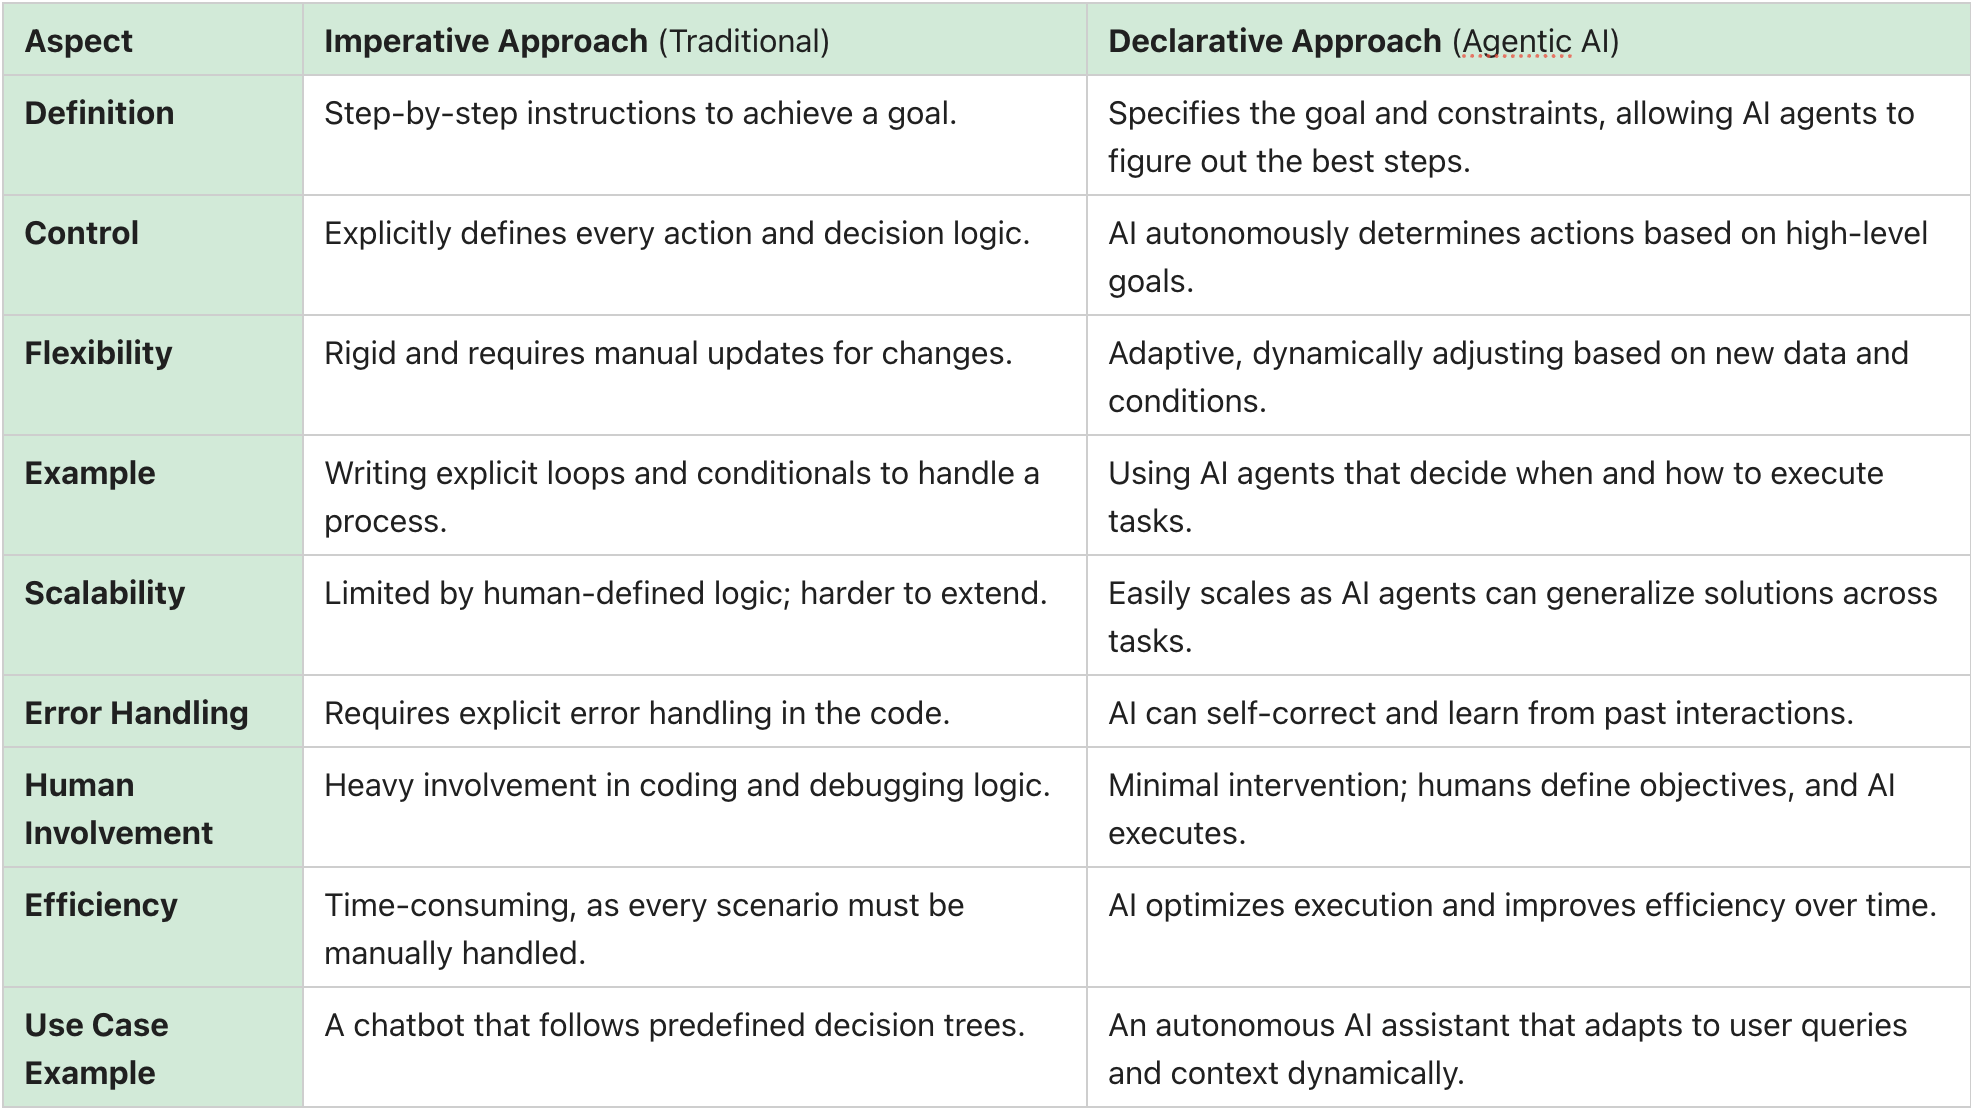
\includegraphics[width=0.9\textwidth]{Images/imperative_declarative_approach.png}
    \captionof{figure}{Imperative vs. Agentic Approach Comparison} \cite{agenticTable}
    \label{fig:agentic-table}
\end{center}


% Technical Background
\section{Technical Background}
This section provides an overview of key technologies enabling the platform's intelligent functionalities.

% Large Language Models (LLMs)
\subsection{Large Language Models (LLMs)}

\subsubsection{Introduction}
Language serves as the cornerstone of human interaction, significantly impacting how humans interface with machines. The evolution of Natural Language Processing (NLP), from early statistical approaches to sophisticated neural architectures, has culminated in the advent of Large Language Models (LLMs). These advancements have been driven by the introduction of transformer-based architectures, substantial improvements in computational resources, and vast amounts of training data. The resulting models exhibit near-human performance in numerous linguistic tasks such as translation, summarization, and conversational dialogues.

\begin{center}
    \centering
    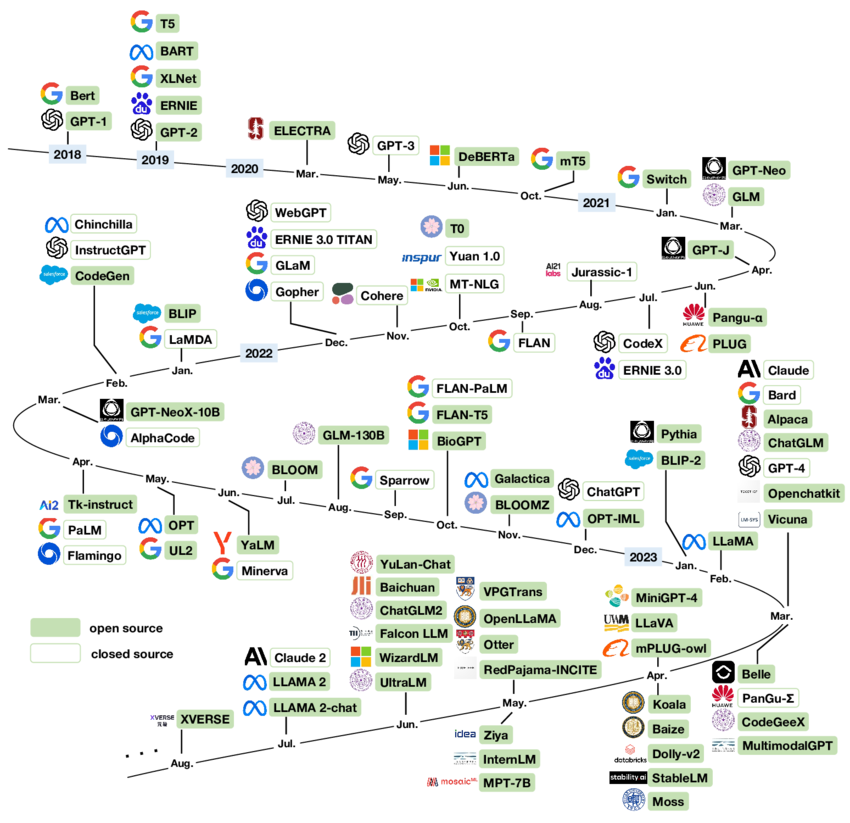
\includegraphics[width=0.9\textwidth]{Images/evolution chronologic LLM.png}
    \captionof{figure}{Chronological Evolution of Large Language Models (LLMs)} \cite{llmEvolution}
    \label{fig:llmEvolution}
\end{center}

\subsubsection{Capabilities and Emergent Properties}
Large Language Models have significantly evolved, exhibiting capabilities such as reasoning, decision-making, and in-context learning, often emerging spontaneously at scale rather than through explicit programming or training. These emergent properties enable LLMs to effectively generalize across diverse tasks without extensive task-specific data, highlighting their robust adaptability. Techniques such as fine-tuning and prompt engineering further enhance model alignment, ensuring outputs align closely with user intents and expectations.\mynewline

LLMs’ adaptability and versatility have found applications in various sectors including healthcare, finance, legal operations, and customer service, underscoring their transformative potential across industries.

\subsubsection{Challenges and Limitations}
Despite these advancements, LLM deployment is constrained by several critical limitations. Key challenges include:

\begin{itemize}
    \item \textbf{Computational Cost and Efficiency}: The resource-intensive nature of LLM training and inference demands considerable computational power, resulting in high operational costs.
    \item \textbf{Input Size Constraints}: Current LLM architectures typically handle context windows of up to 128k tokens, limiting their ability to directly process large-scale data sources comprising millions of tokens.
    \item \textbf{Inference Speed and Latency}: Longer inputs proportionally increase inference time and computational demands, challenging real-time or large-scale applications.
    \item \textbf{Ethical and Bias Considerations}: Models may inadvertently propagate biases present in training data or generate misleading and potentially harmful outputs, necessitating robust ethical oversight.
\end{itemize}

Figures~\ref{fig:llmSpeedComparison}, \ref{fig:llmPriceComparison}, and \ref{fig:llmIntelligenceComparison} summarize comparative metrics across popular LLMs, highlighting trade-offs in performance, cost, and processing speed.

\begin{center}
    \centering
    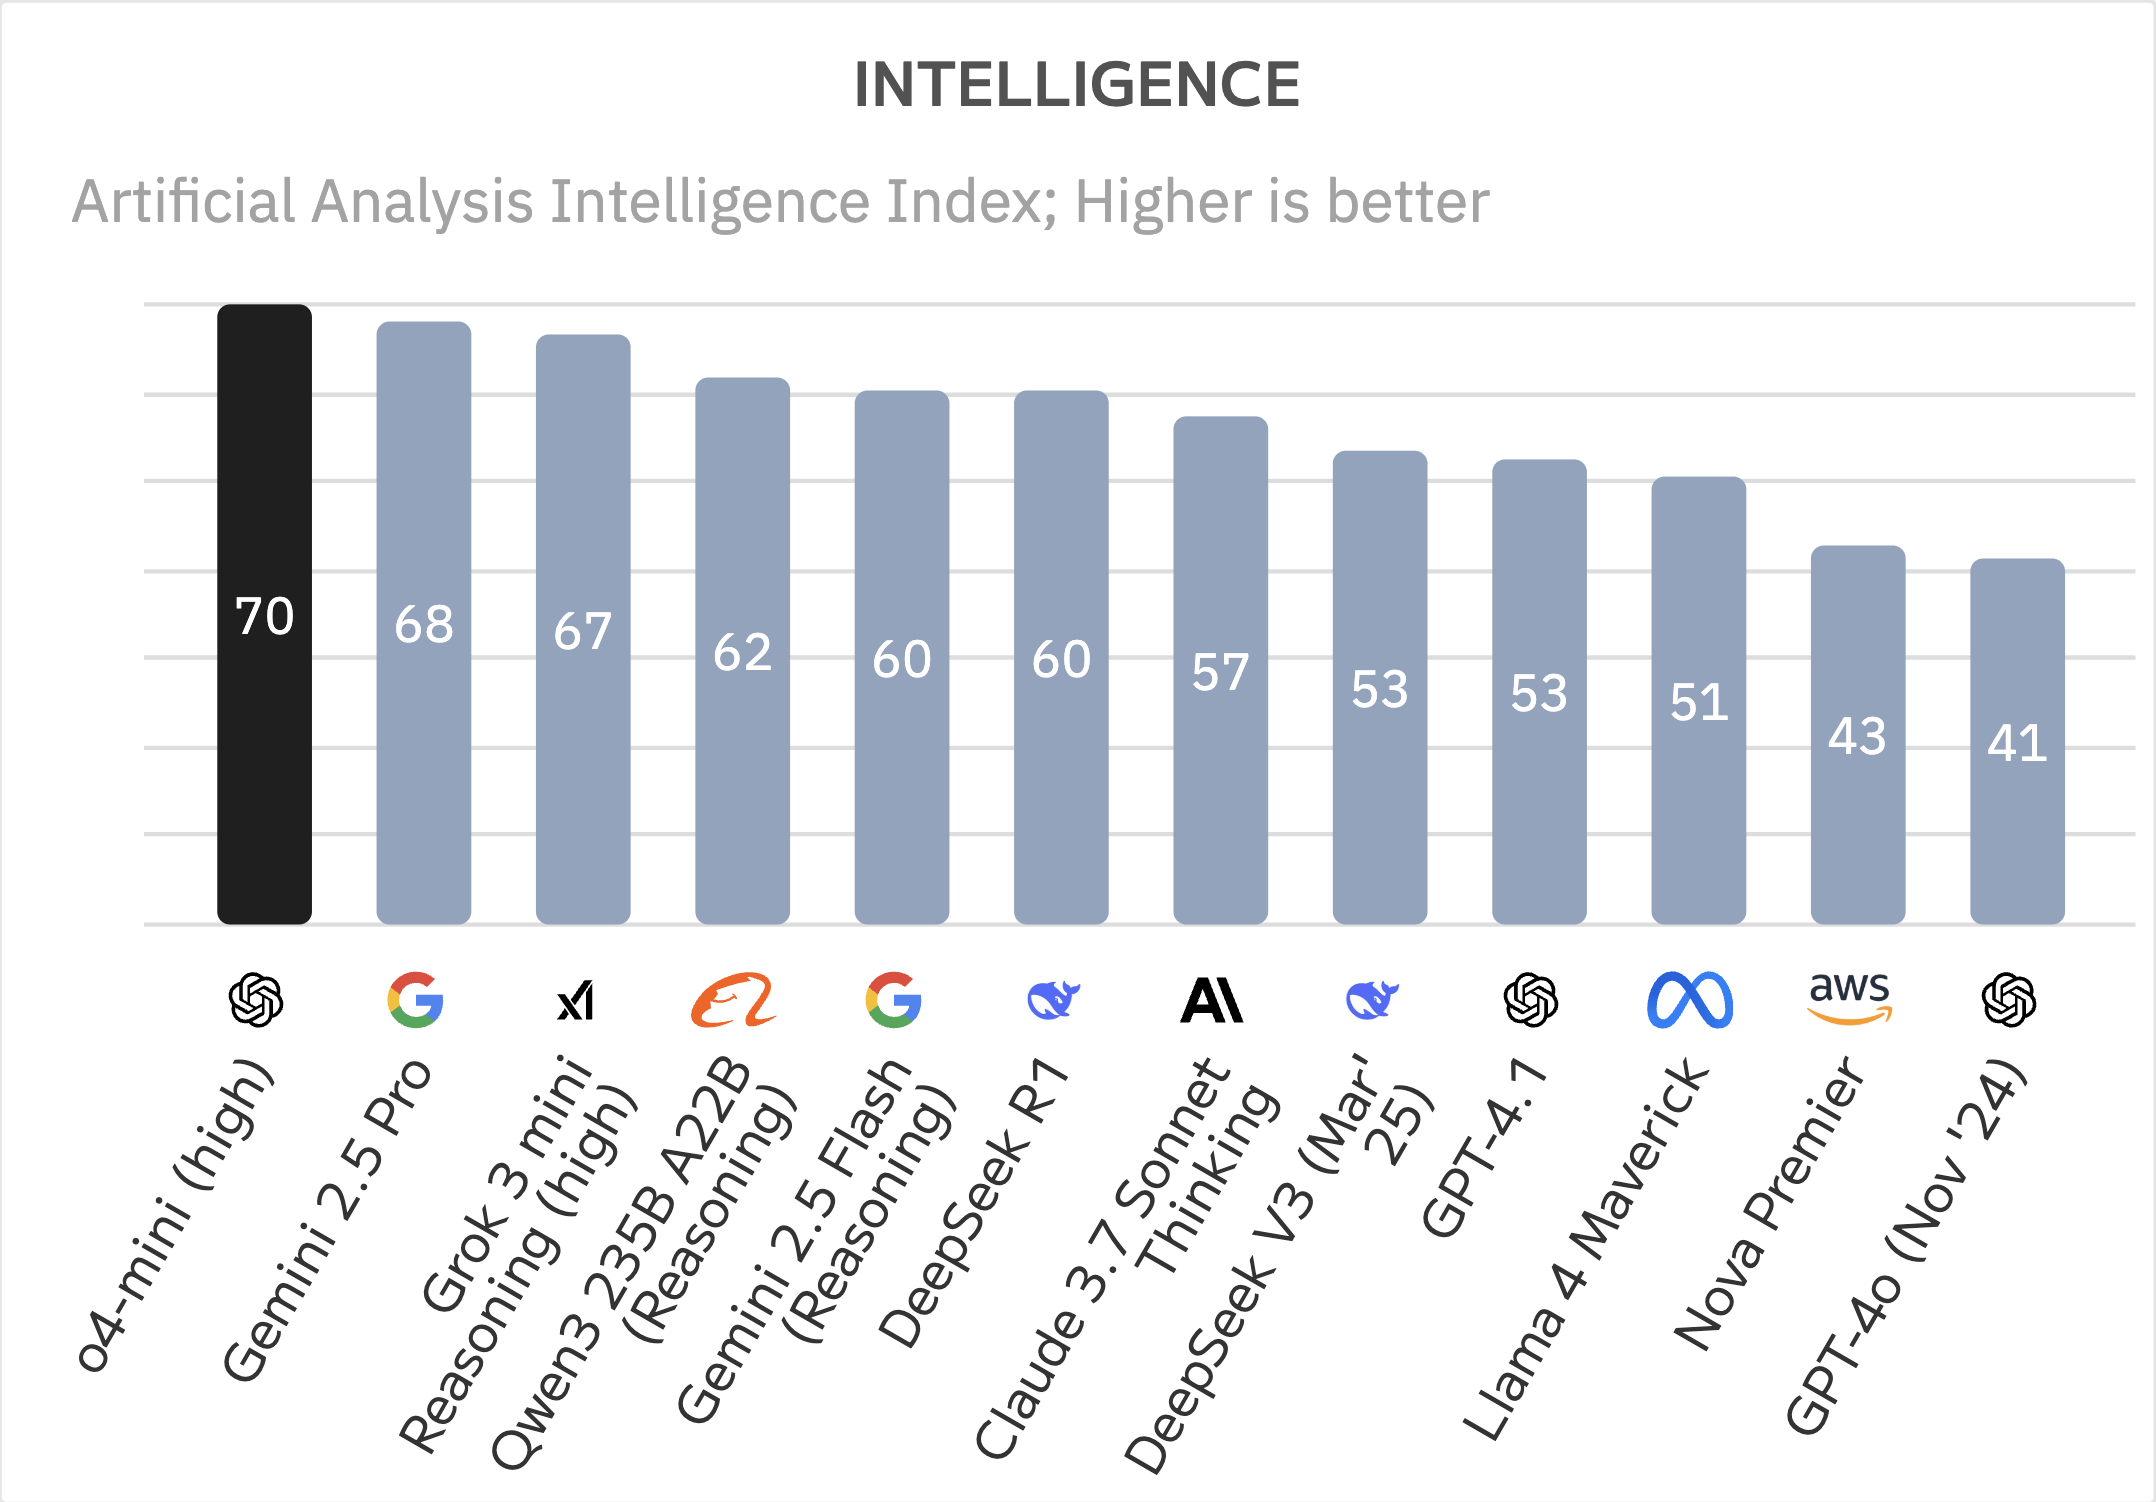
\includegraphics[width=0.85\textwidth]{Images/inteligence_LLM_comparison.png}
    \captionof{figure}{Comparative Intelligence Index of LLMs} \cite{llmIntelligenceComparison}
    \label{fig:llmIntelligenceComparison}
\end{center}

\begin{center}
    \centering
    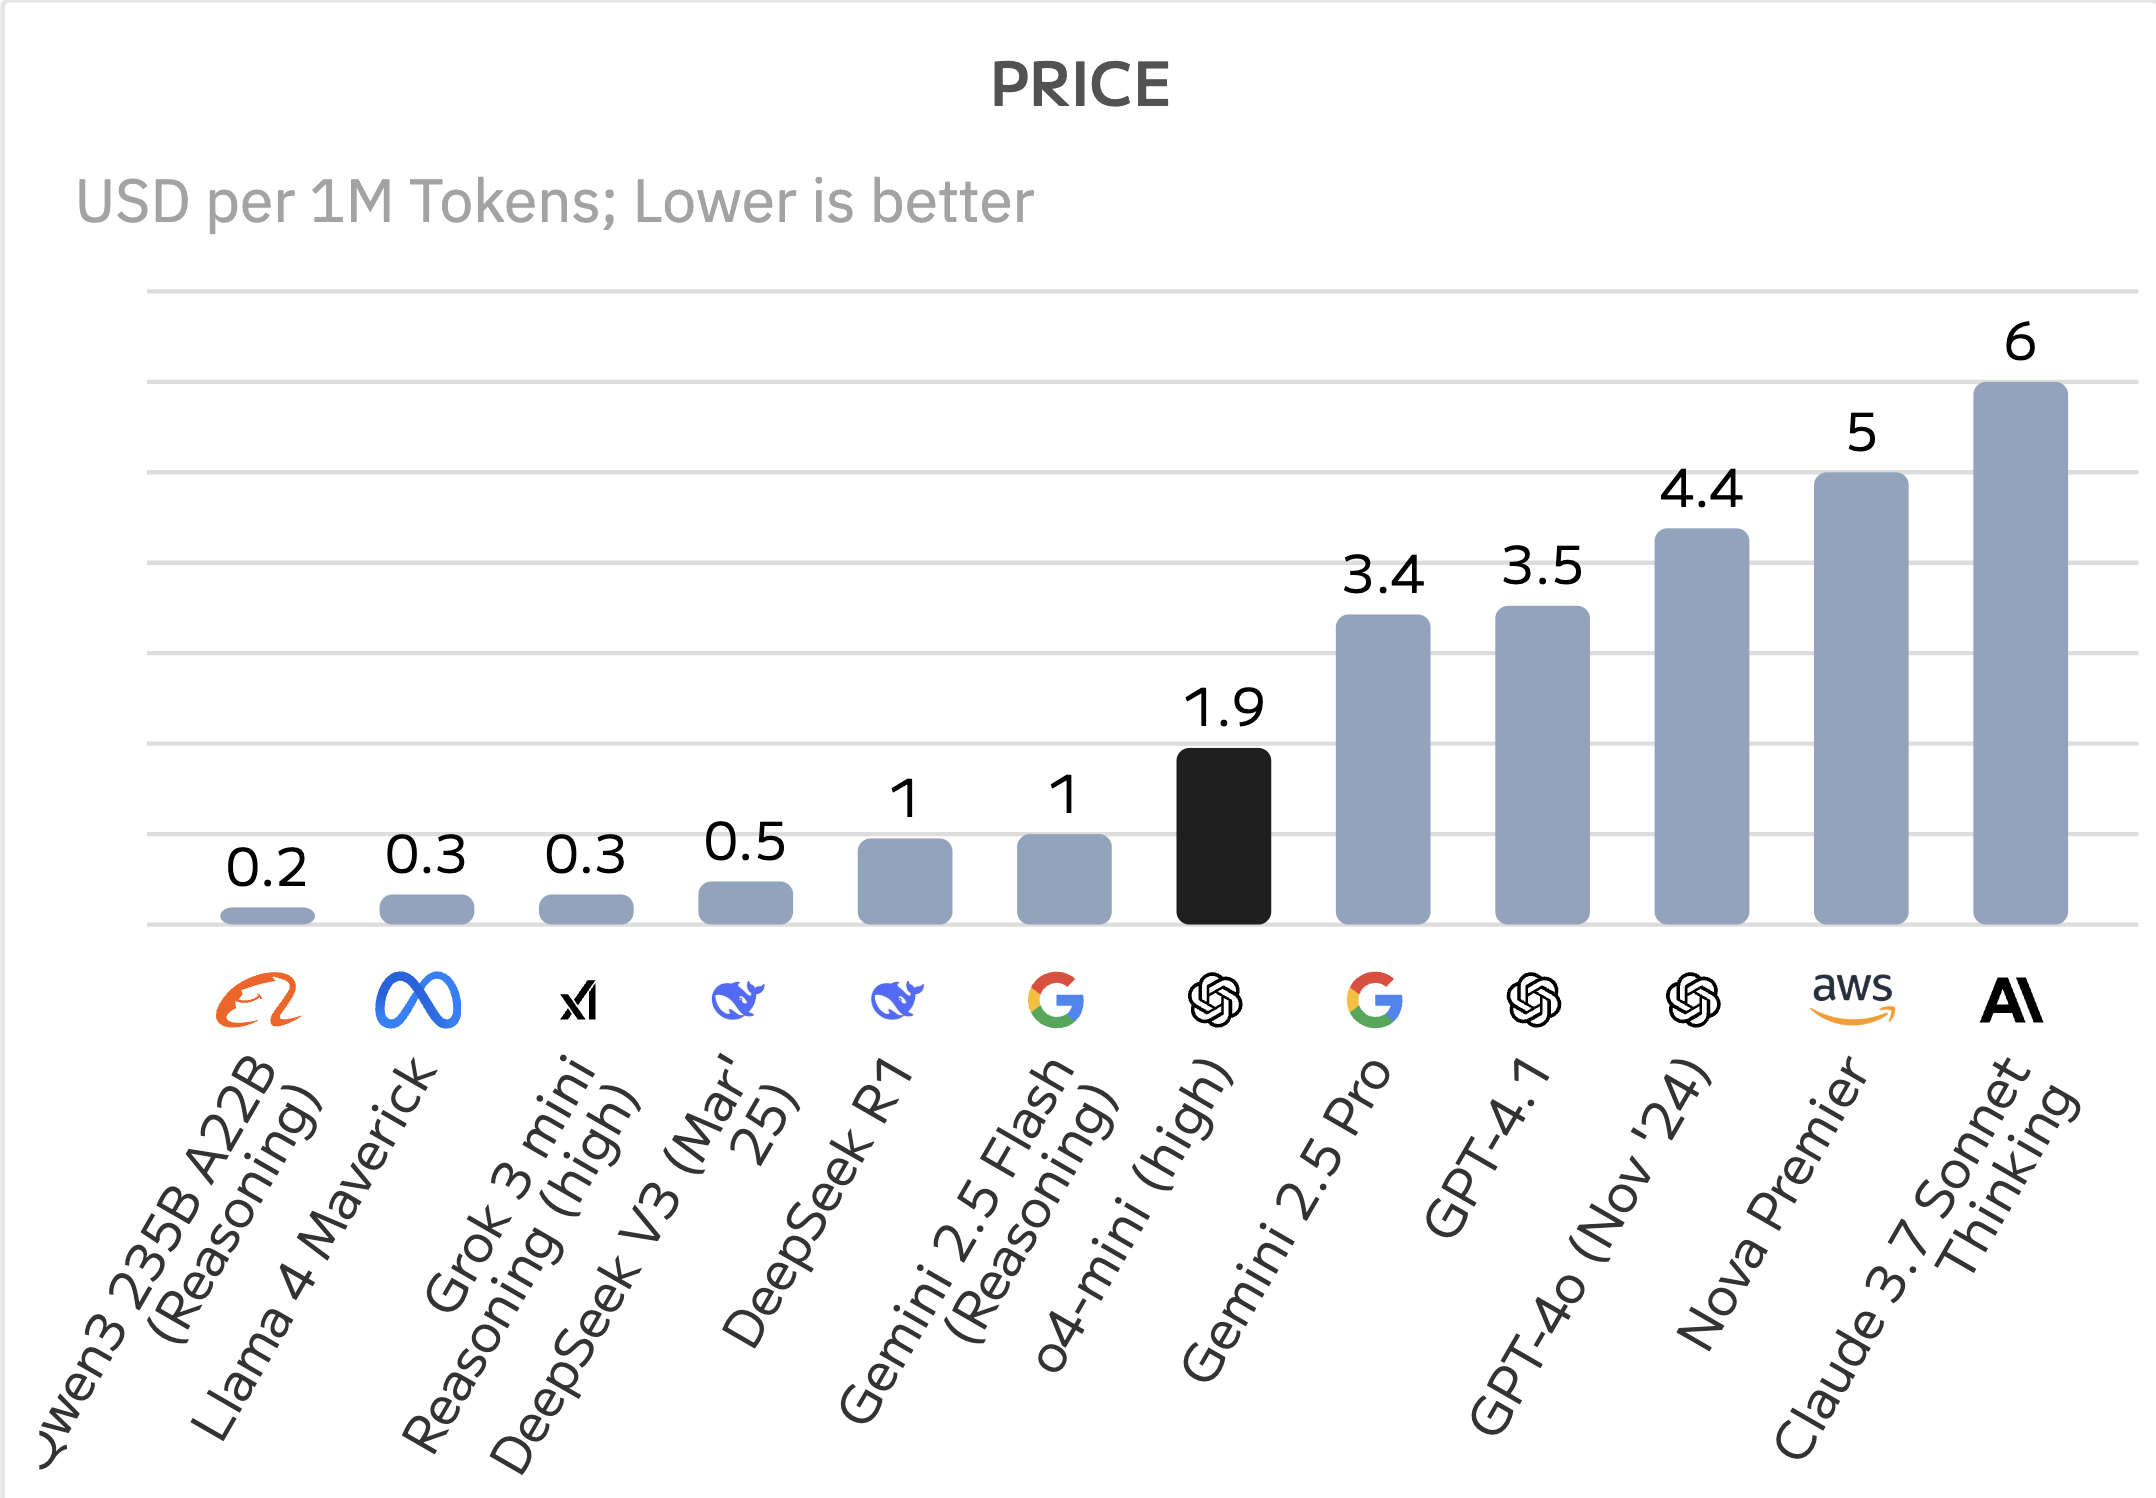
\includegraphics[width=0.85\textwidth]{Images/price_LLM_comparison.png}
    \captionof{figure}{Cost Comparison per Million Tokens} \cite{llmPriceComparison}
    \label{fig:llmPriceComparison}
\end{center}

\begin{center}
    \centering
    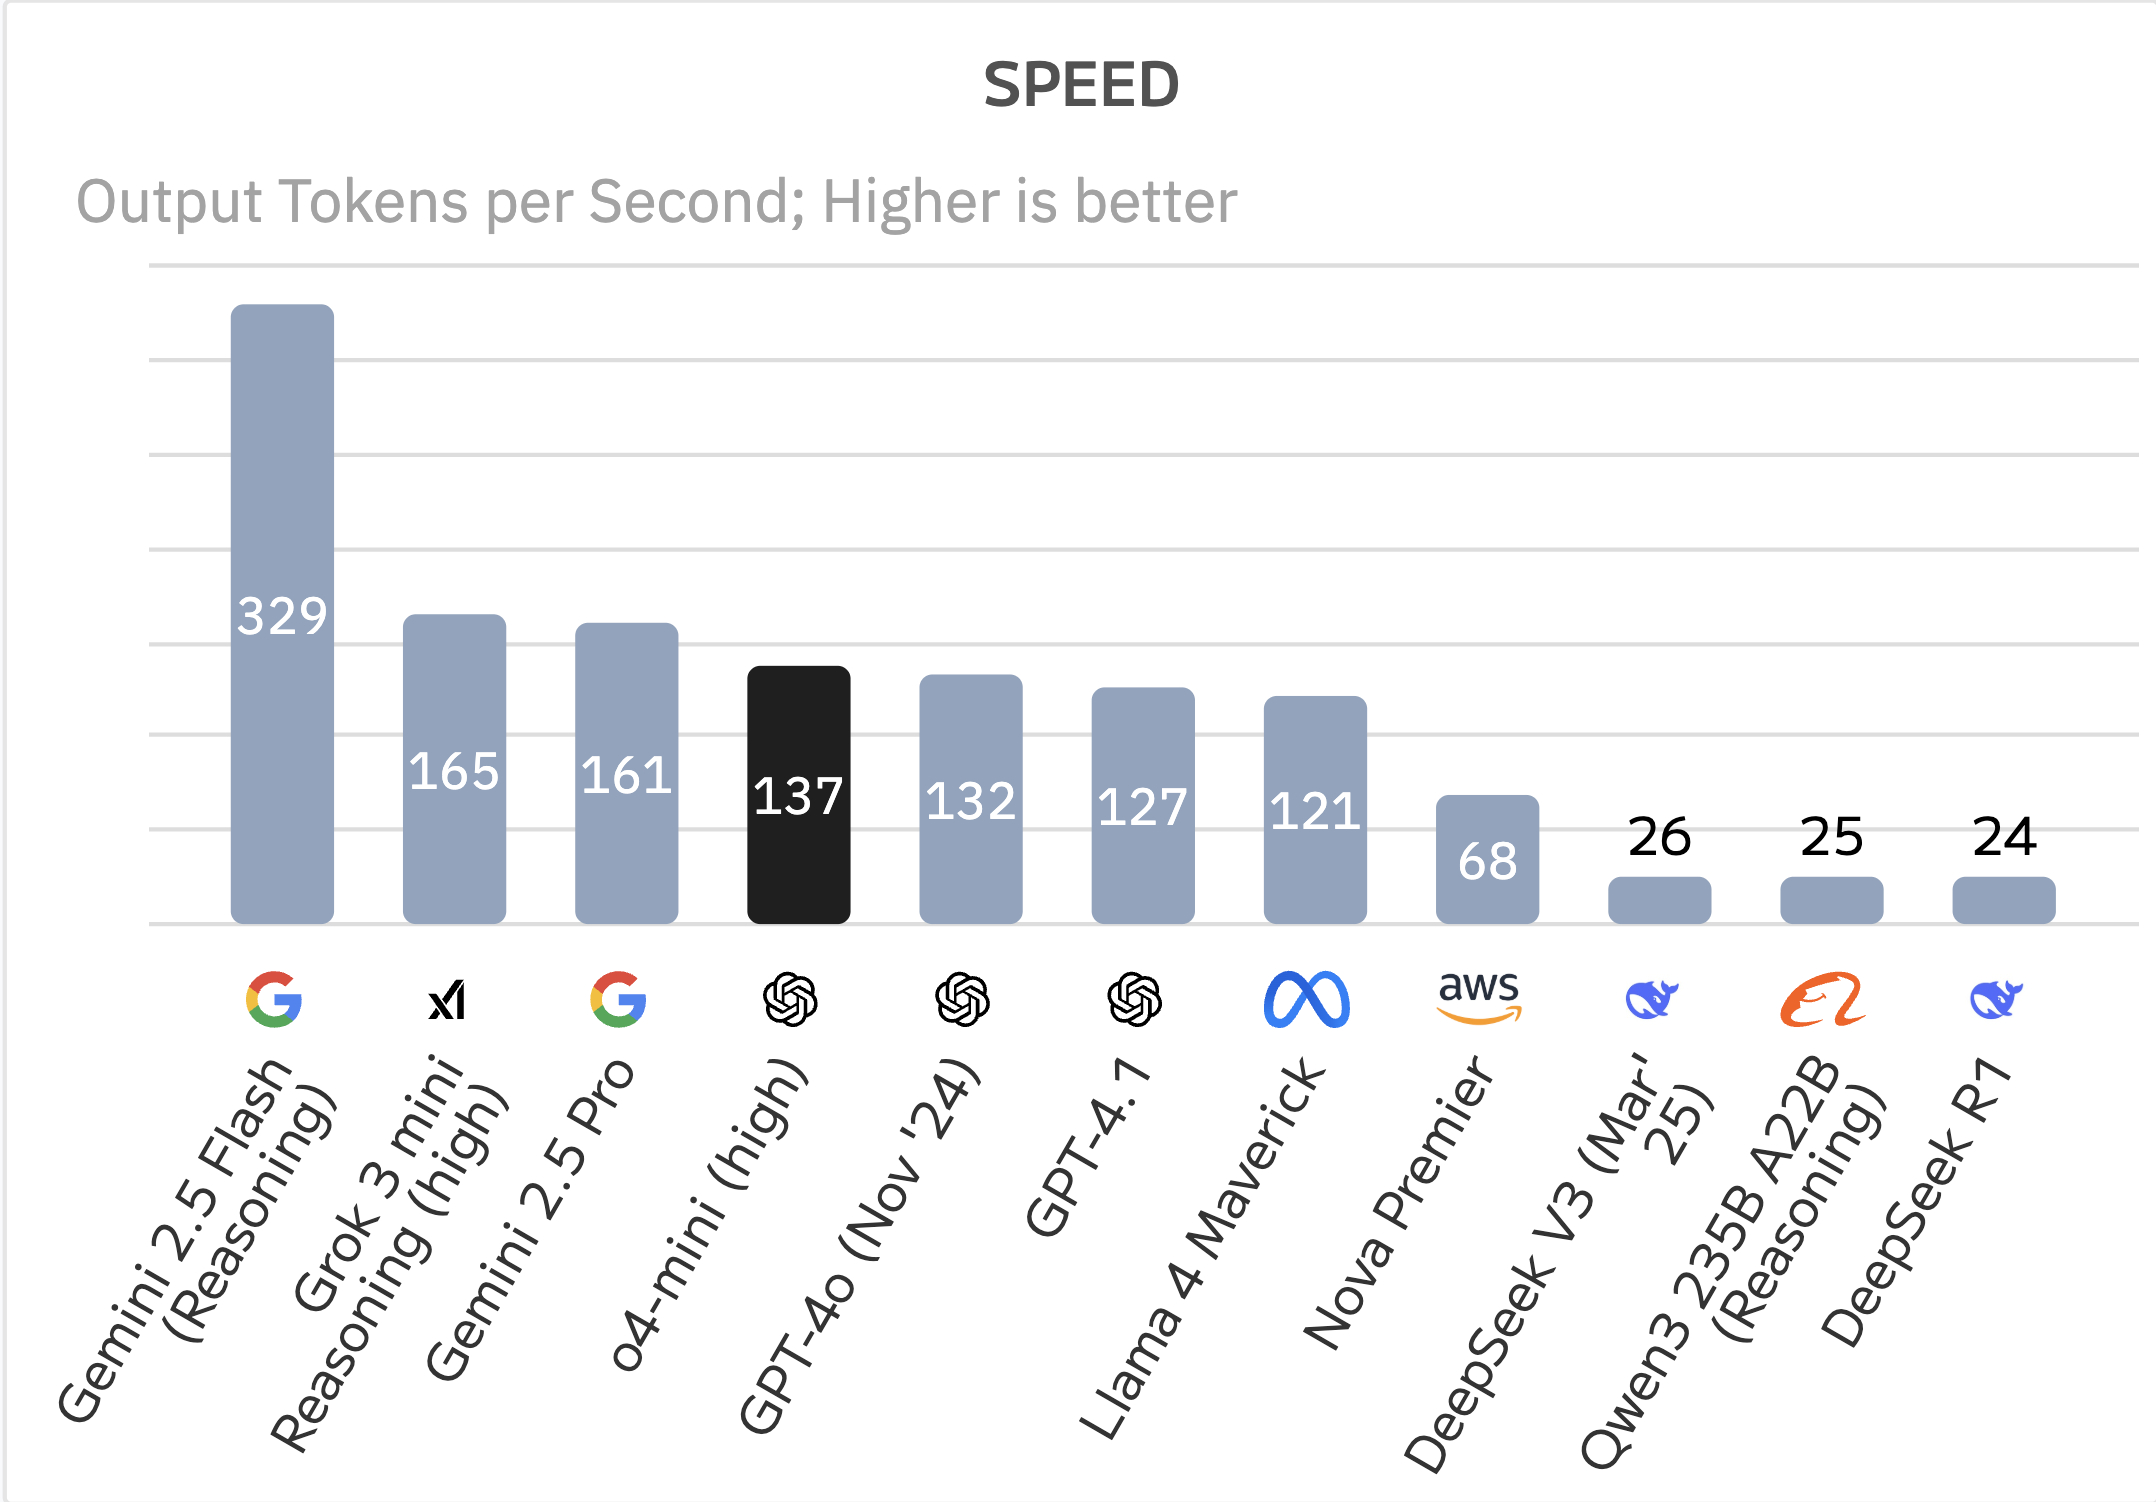
\includegraphics[width=0.85\textwidth]{Images/speed_LLM_comparison.png}
    \captionof{figure}{Inference Speed Comparison of Various LLMs} \cite{llmSpeedComparison}
    \label{fig:llmSpeedComparison}
\end{center}

\subsubsection{Future Directions}
Addressing these constraints has become an active area of research. Innovations in model compression techniques, such as pruning, quantization, and distillation, aim to enhance efficiency and accessibility of LLMs. Moreover, emerging architectures and retrieval-augmented generation methods offer promising approaches for handling extensive datasets and large input contexts effectively.

Future advancements are expected to mitigate current limitations, further unlocking the full potential of Large Language Models across diverse, complex applications.

% Agentic AI
\subsection{Agentic AI}

\subsubsection{Introduction}
Agentic AI represents a significant evolution in artificial intelligence, transitioning from reactive systems to proactive, autonomous entities capable of setting goals, making decisions, and adapting to dynamic environments. Unlike traditional AI agents that operate within predefined parameters, Agentic AI systems exhibit autonomy, learning, and adaptability, enabling them to handle complex, multi-step tasks with minimal human intervention.

\begin{center}
    \centering
    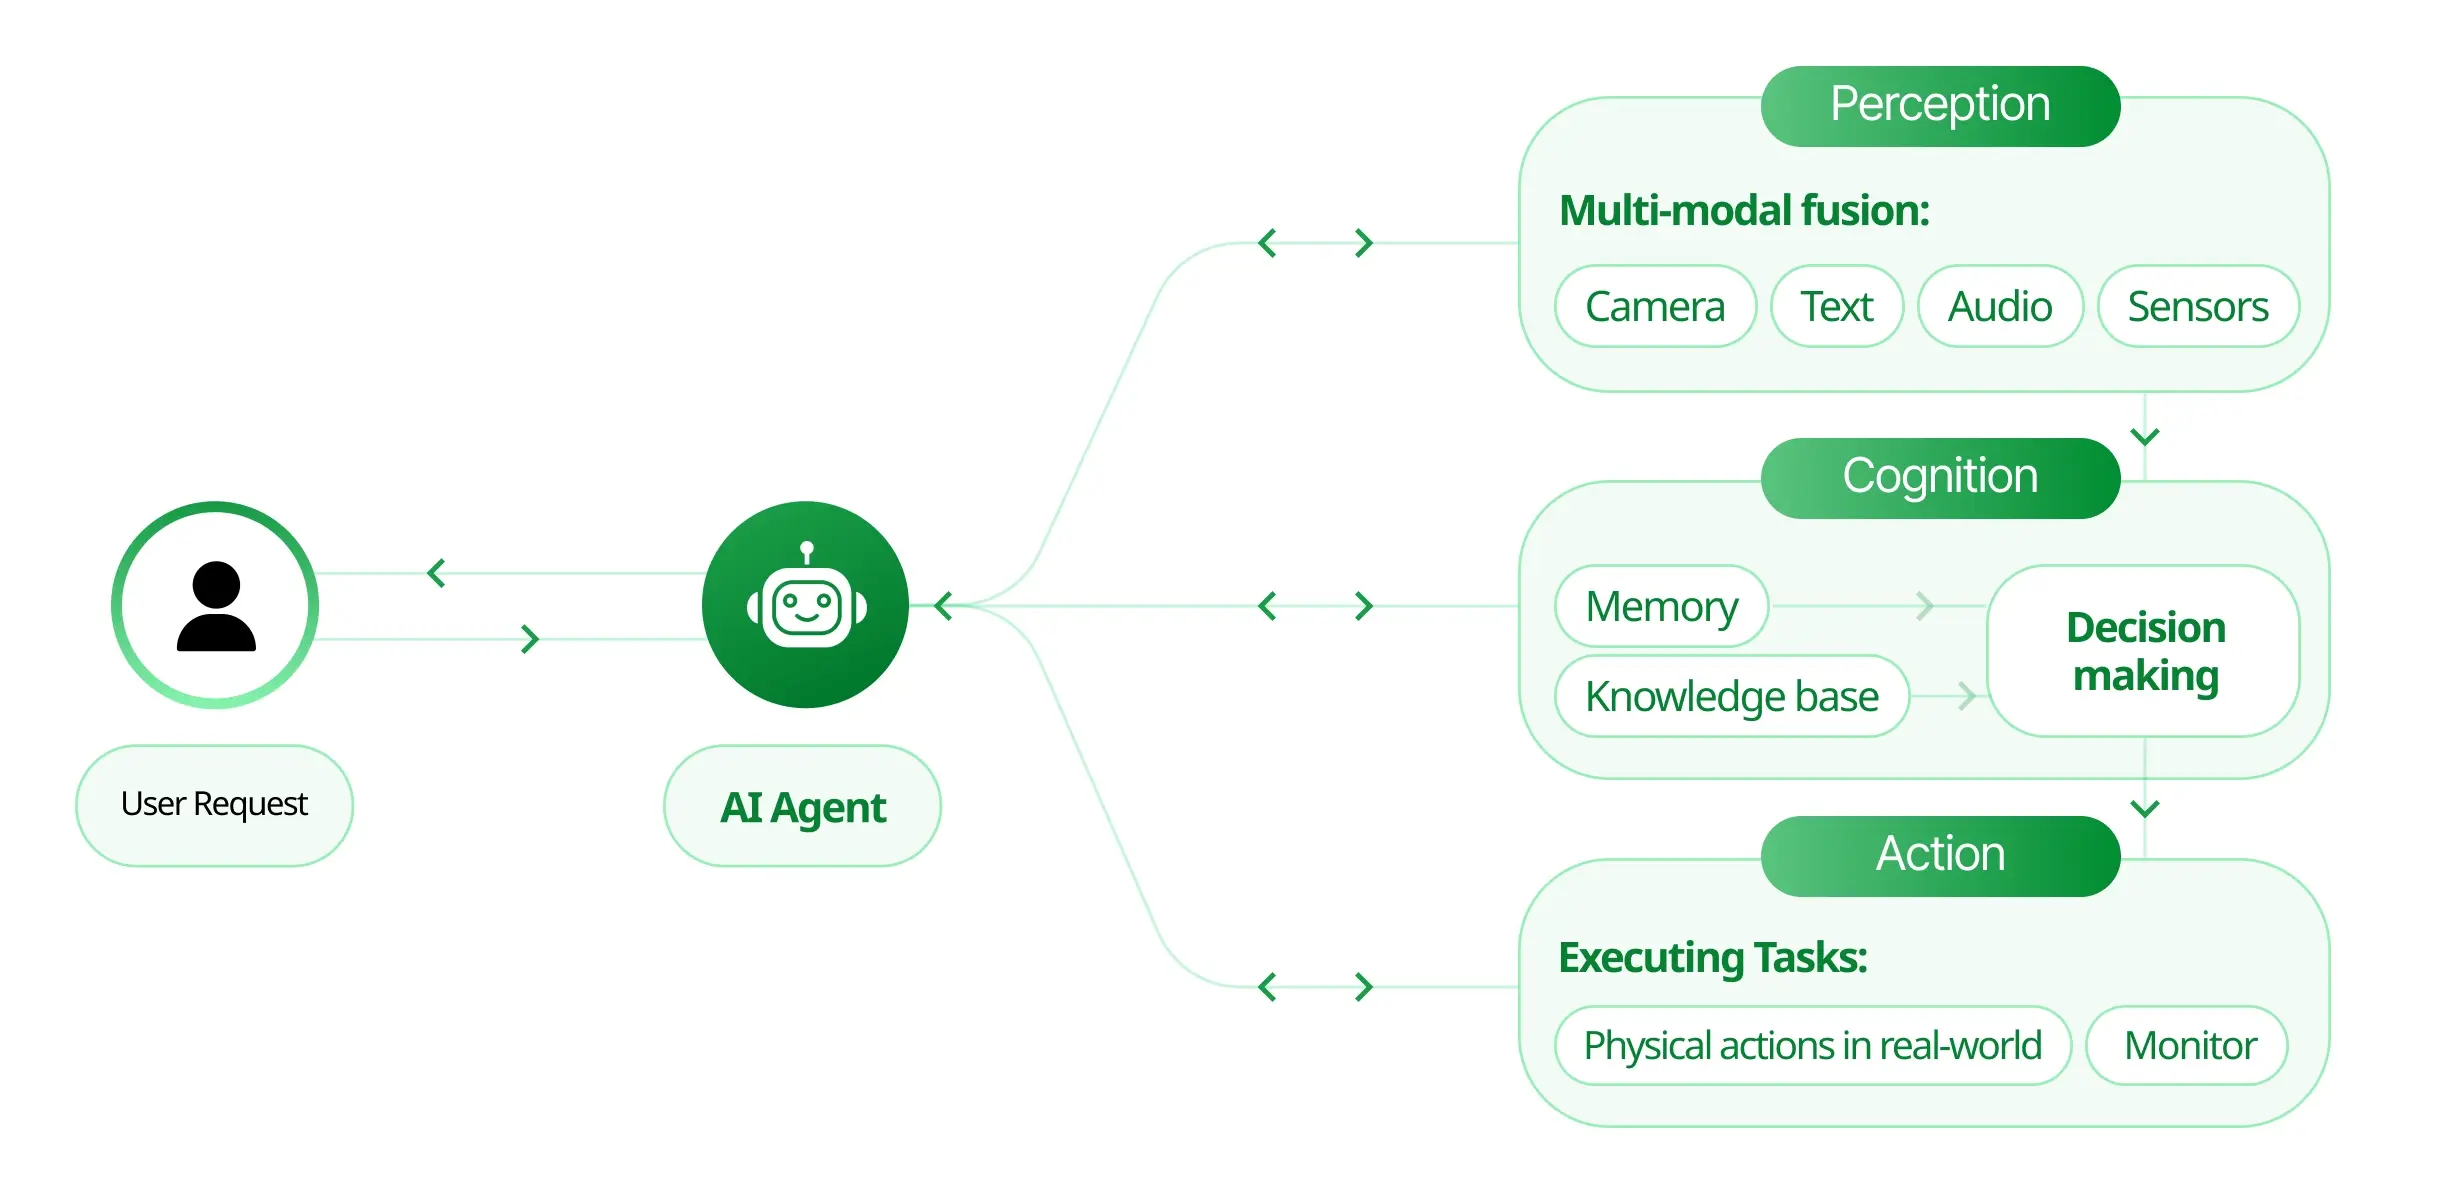
\includegraphics[width=0.9\textwidth]{Images/agentic_ai_architecture.png}
    \captionof{figure}{Agentic AI System Architecture} \cite{agenticAIArchitecture}
    \label{fig:agentic_ai_architecture}
\end{center}

\subsubsection{Core Characteristics}
Agentic AI systems are distinguished by several key features:

\begin{itemize}
    \item \textbf{Autonomy}: They operate independently, making decisions without continuous human oversight.
    \item \textbf{Goal-Oriented Behavior}: These systems can set, pursue, and adjust goals based on environmental feedback.
    \item \textbf{Adaptability}: Agentic AI learns from experiences, refining its strategies to improve performance over time.
    \item \textbf{Complex Decision-Making}: They evaluate multiple options and potential outcomes to make informed decisions.
    \item \textbf{Collaboration}: Agentic AI can coordinate with other agents or systems to achieve shared objectives.
\end{itemize}

\subsubsection{Agentic AI vs. Generative AI}
While both Agentic AI and Generative AI leverage advanced machine learning techniques, their functionalities differ significantly:

\begin{itemize}
    \item \textbf{Generative AI}: Focuses on creating content (text, images, etc.) based on input data, operating primarily in a reactive manner.
    \item \textbf{Agentic AI}: Emphasizes autonomous decision-making and goal pursuit, enabling proactive interactions with the environment.
\end{itemize}

\begin{center}
    \centering
    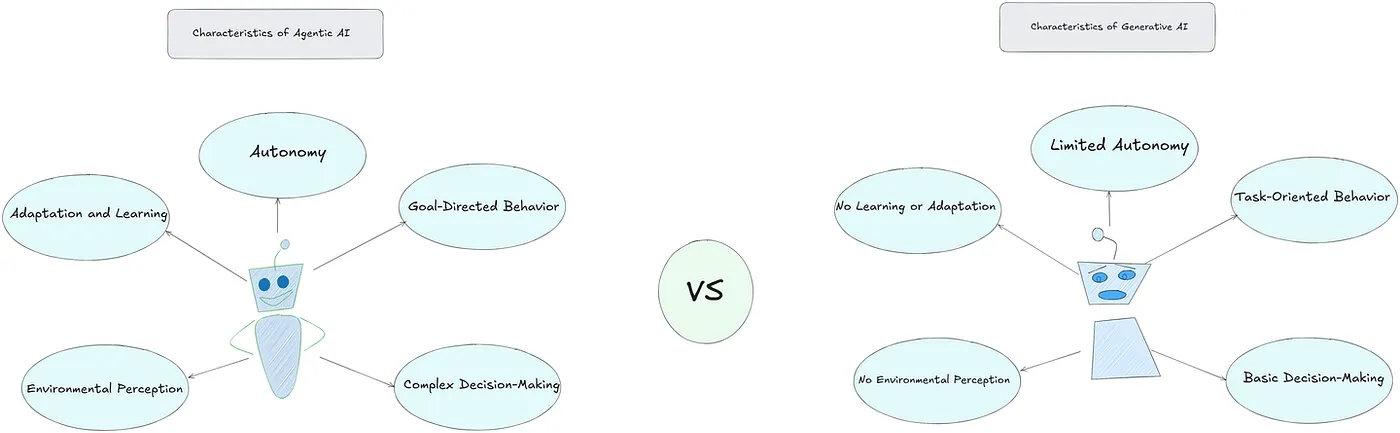
\includegraphics[width=0.9\textwidth]{Images/agentic_vs_generative_ai.png}
    \captionof{figure}{Comparison Between Agentic AI and Generative AI} \cite{agenticAIvsGenerativeAI}
    \label{fig:agentic_vs_generative_ai}
\end{center}

\subsubsection{Multi-Agent Systems}
Agentic AI often operates within multi-agent systems, where multiple autonomous agents collaborate to solve complex problems. These systems benefit from:

\begin{itemize}
    \item \textbf{Specialization}: Agents can focus on specific tasks, enhancing efficiency.
    \item \textbf{Scalability}: Systems can be expanded by adding more agents to handle increased complexity.
    \item \textbf{Robustness}: Collaboration among agents can compensate for individual agent failures or limitations.
\end{itemize}

\begin{center}
    \centering
    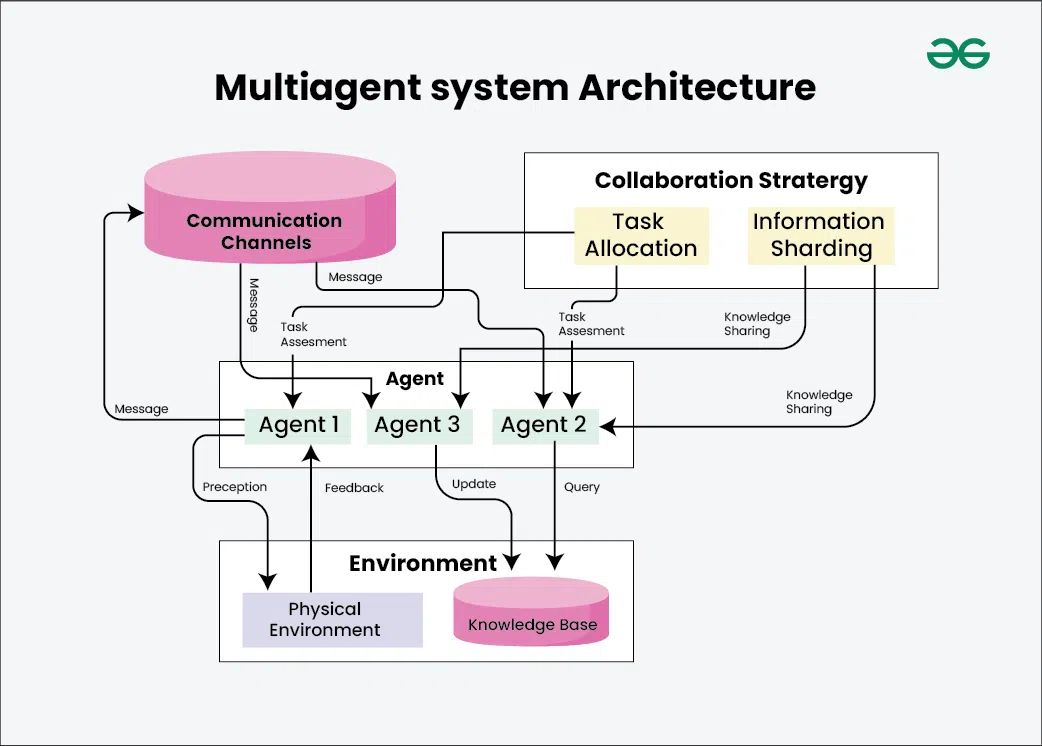
\includegraphics[width=0.9\textwidth]{Images/multi_agent_system.png}
    \captionof{figure}{Multi-Agent System Collaboration} \cite{multiAgentSystem}
    \label{fig:multi_agent_system}
\end{center}

\subsubsection{Applications of Agentic AI}
Agentic AI has diverse applications across various industries:

\begin{itemize}
    \item \textbf{Healthcare}: Assisting in diagnostics, treatment planning, and patient monitoring.
    \item \textbf{Finance}: Managing portfolios, detecting fraud, and optimizing trading strategies.
    \item \textbf{Manufacturing}: Overseeing production lines, predicting maintenance needs, and ensuring quality control.
    \item \textbf{Transportation}: Enabling autonomous vehicles to navigate and make real-time decisions.
    \item \textbf{Customer Service}: Providing personalized support through adaptive virtual assistants.
\end{itemize}

\subsubsection{Challenges and Future Directions}
Despite its potential, Agentic AI faces several challenges:

\begin{itemize}
    \item \textbf{Ethical Considerations}: Ensuring decisions align with human values and societal norms.
    \item \textbf{Transparency}: Making decision-making processes understandable to users.
    \item \textbf{Security}: Protecting systems from malicious manipulation or unintended behaviors.
    \item \textbf{Integration}: Seamlessly incorporating Agentic AI into existing infrastructures.
\end{itemize}

Ongoing research aims to address these challenges, focusing on developing frameworks for ethical AI, enhancing interpretability, and establishing standards for safe deployment.

% Modular Component Platform (MCP)
\subsection{Model Context Protocol (MCP)}

% Introduction
\subsubsection{Introduction}
The Model Context Protocol (MCP) is an open standard developed by Anthropic in late 2024 to address the growing complexity of integrating large language models (LLMs) with diverse external tools, systems, and data sources. MCP provides a standardized interface that enables AI applications to interact seamlessly with various resources, facilitating context exchange and enhancing the capabilities of AI assistants.

\begin{center}
    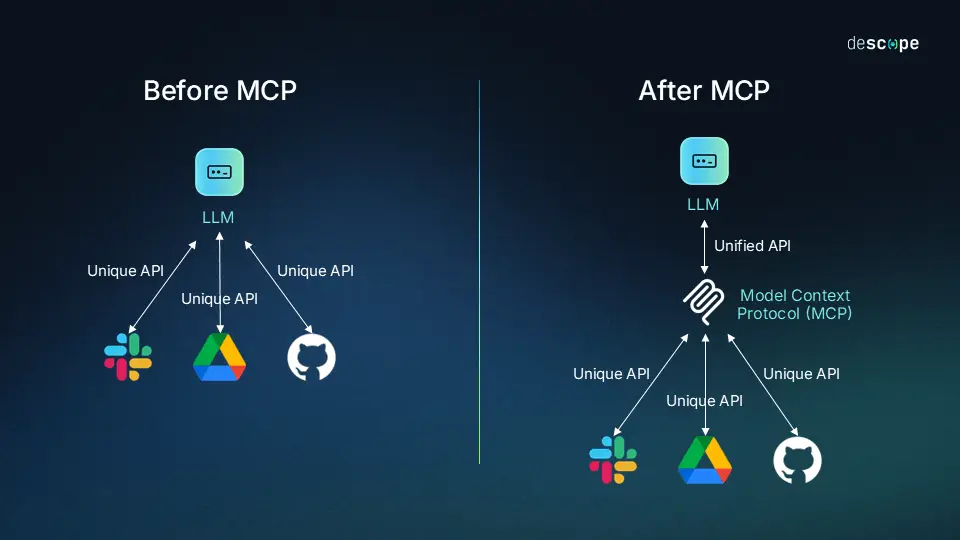
\includegraphics[width=0.9\textwidth]{Images/before_and_after_mcp.png}
    \captionof{figure}{Before and After Model Context Protocol (MCP)} \cite{mcpBeforeAfter}
    \label{fig:mcp_before_after}
\end{center}

% Architecture
\subsubsection{Architecture}
MCP follows a client-host-server architecture, where:

\begin{itemize}
    \item \textbf{Hosts} are LLM applications (e.g., Claude Desktop, IDEs) that initiate connections.
    \item \textbf{Clients} maintain 1:1 connections with servers within the host application.
    \item \textbf{Servers} provide context, tools, and prompts to clients.
\end{itemize}

This architecture allows for modular integration, enabling AI systems to access and utilize external resources efficiently.

\begin{center}
    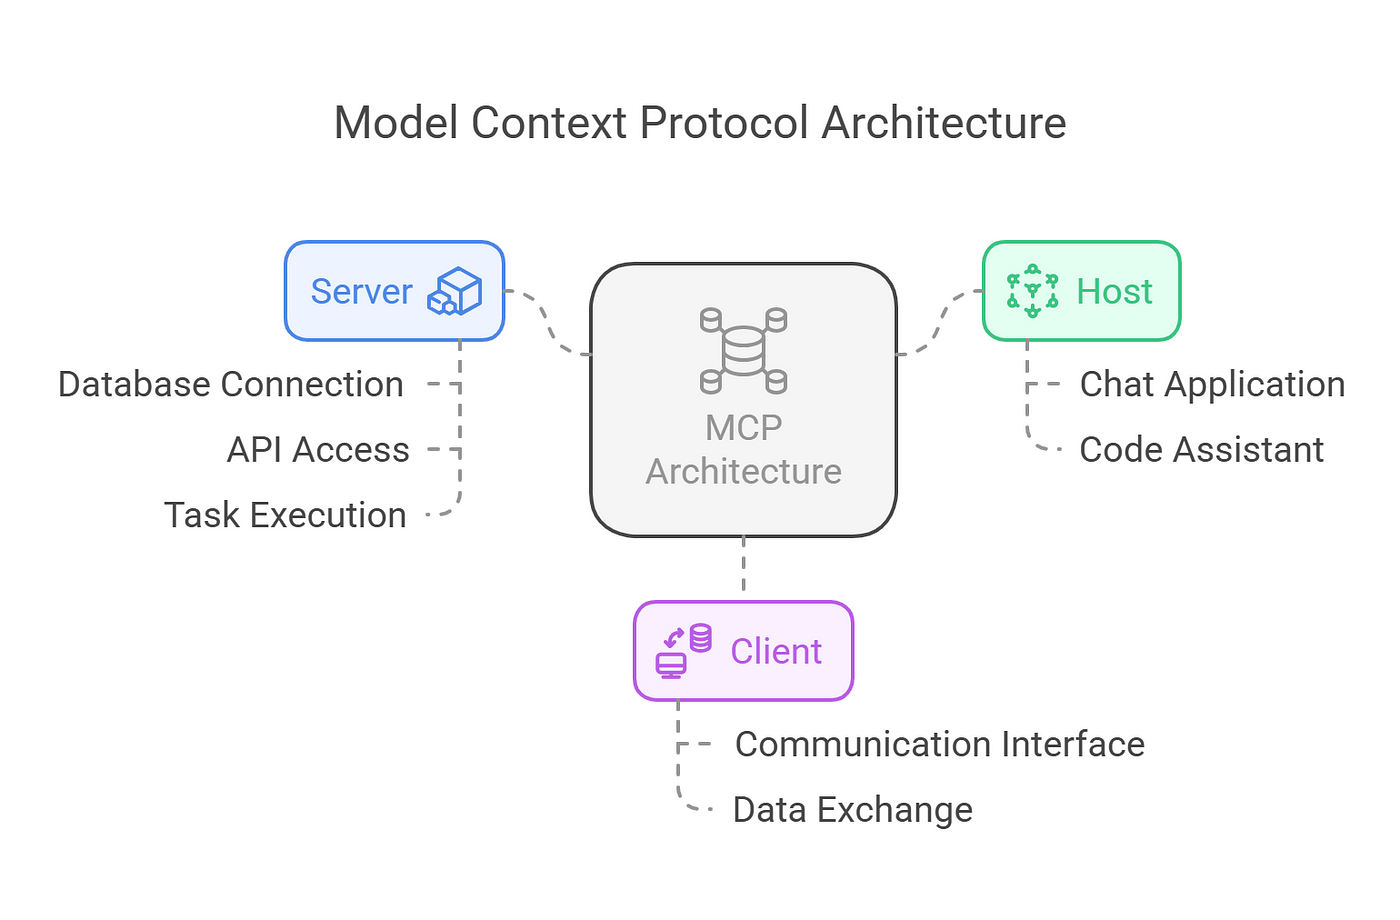
\includegraphics[width=0.9\textwidth]{Images/mcp_architecture_diagram.png}
    \captionof{figure}{Model Context Protocol Architecture} \cite{mcpArchitecture}
    \label{fig:mcp_architecture}
\end{center}

% Core Components
\subsubsection{Core Components}
MCP servers can expose three main types of capabilities:

\begin{itemize}
    \item \textbf{Resources}: File-like data that can be read by clients (e.g., API responses, file contents).
    \item \textbf{Tools}: Functions that can be called by the LLM with user approval.
    \item \textbf{Prompts}: Pre-written templates that assist users in accomplishing specific tasks.
\end{itemize}

These components enable AI assistants to perform complex tasks by leveraging external data and functionalities.

% Advantages
\subsubsection{Advantages}
MCP offers several benefits:

\begin{itemize}
    \item \textbf{Standardization}: Provides a universal method for connecting AI assistants to external data sources and systems.
    \item \textbf{Scalability}: Simplifies integration across different AI systems and data, reducing the need for custom connectors.
    \item \textbf{Security}: Facilitates secure interactions between AI applications and local or remote resources.
\end{itemize}

By adopting MCP, developers can enhance the interoperability and efficiency of AI applications.

% Applications
\subsubsection{Applications}
MCP has been applied across various domains:

\begin{itemize}
    \item \textbf{Software Development}: IDEs like Zed and platforms like Replit use MCP to provide coding assistants with real-time code context.
    \item \textbf{Enterprise Assistants}: Companies utilize MCP to allow internal assistants to retrieve information from proprietary documents and systems.
    \item \textbf{Natural Language Data Access}: Applications leverage MCP to connect models with databases, enabling plain-language queries.
\end{itemize}

These applications demonstrate MCP’s versatility in enhancing AI capabilities across different sectors.

% Conclusion
\subsubsection{Conclusion}
The Model Context Protocol represents a significant advancement in AI integration, offering a standardized approach to connect LLMs with external tools and data sources. By facilitating seamless interactions and context exchange, MCP empowers AI applications to perform more complex and context-aware tasks, paving the way for more intelligent and versatile AI systems.

% LangChain and LangGraph
\subsection{LangChain and LangGraph}

\subsubsection{Overview}
LangChain and LangGraph are complementary frameworks designed to facilitate the development of applications powered by Large Language Models (LLMs). While LangChain provides a modular approach to constructing sequential workflows, LangGraph introduces a graph-based paradigm, enabling the creation of complex, dynamic, and stateful AI systems.

\subsubsection{LangChain: Modular Workflow Construction}
LangChain is an open-source framework that simplifies the integration of LLMs into applications by allowing developers to build chains—sequences of calls to LLMs and other utilities. Its modular design supports the composition of various components such as prompt templates, memory modules, and tool integrations. This structure is particularly effective for tasks that follow a linear progression, such as document summarization, question answering, and conversational agents.

\begin{center}
    \centering
    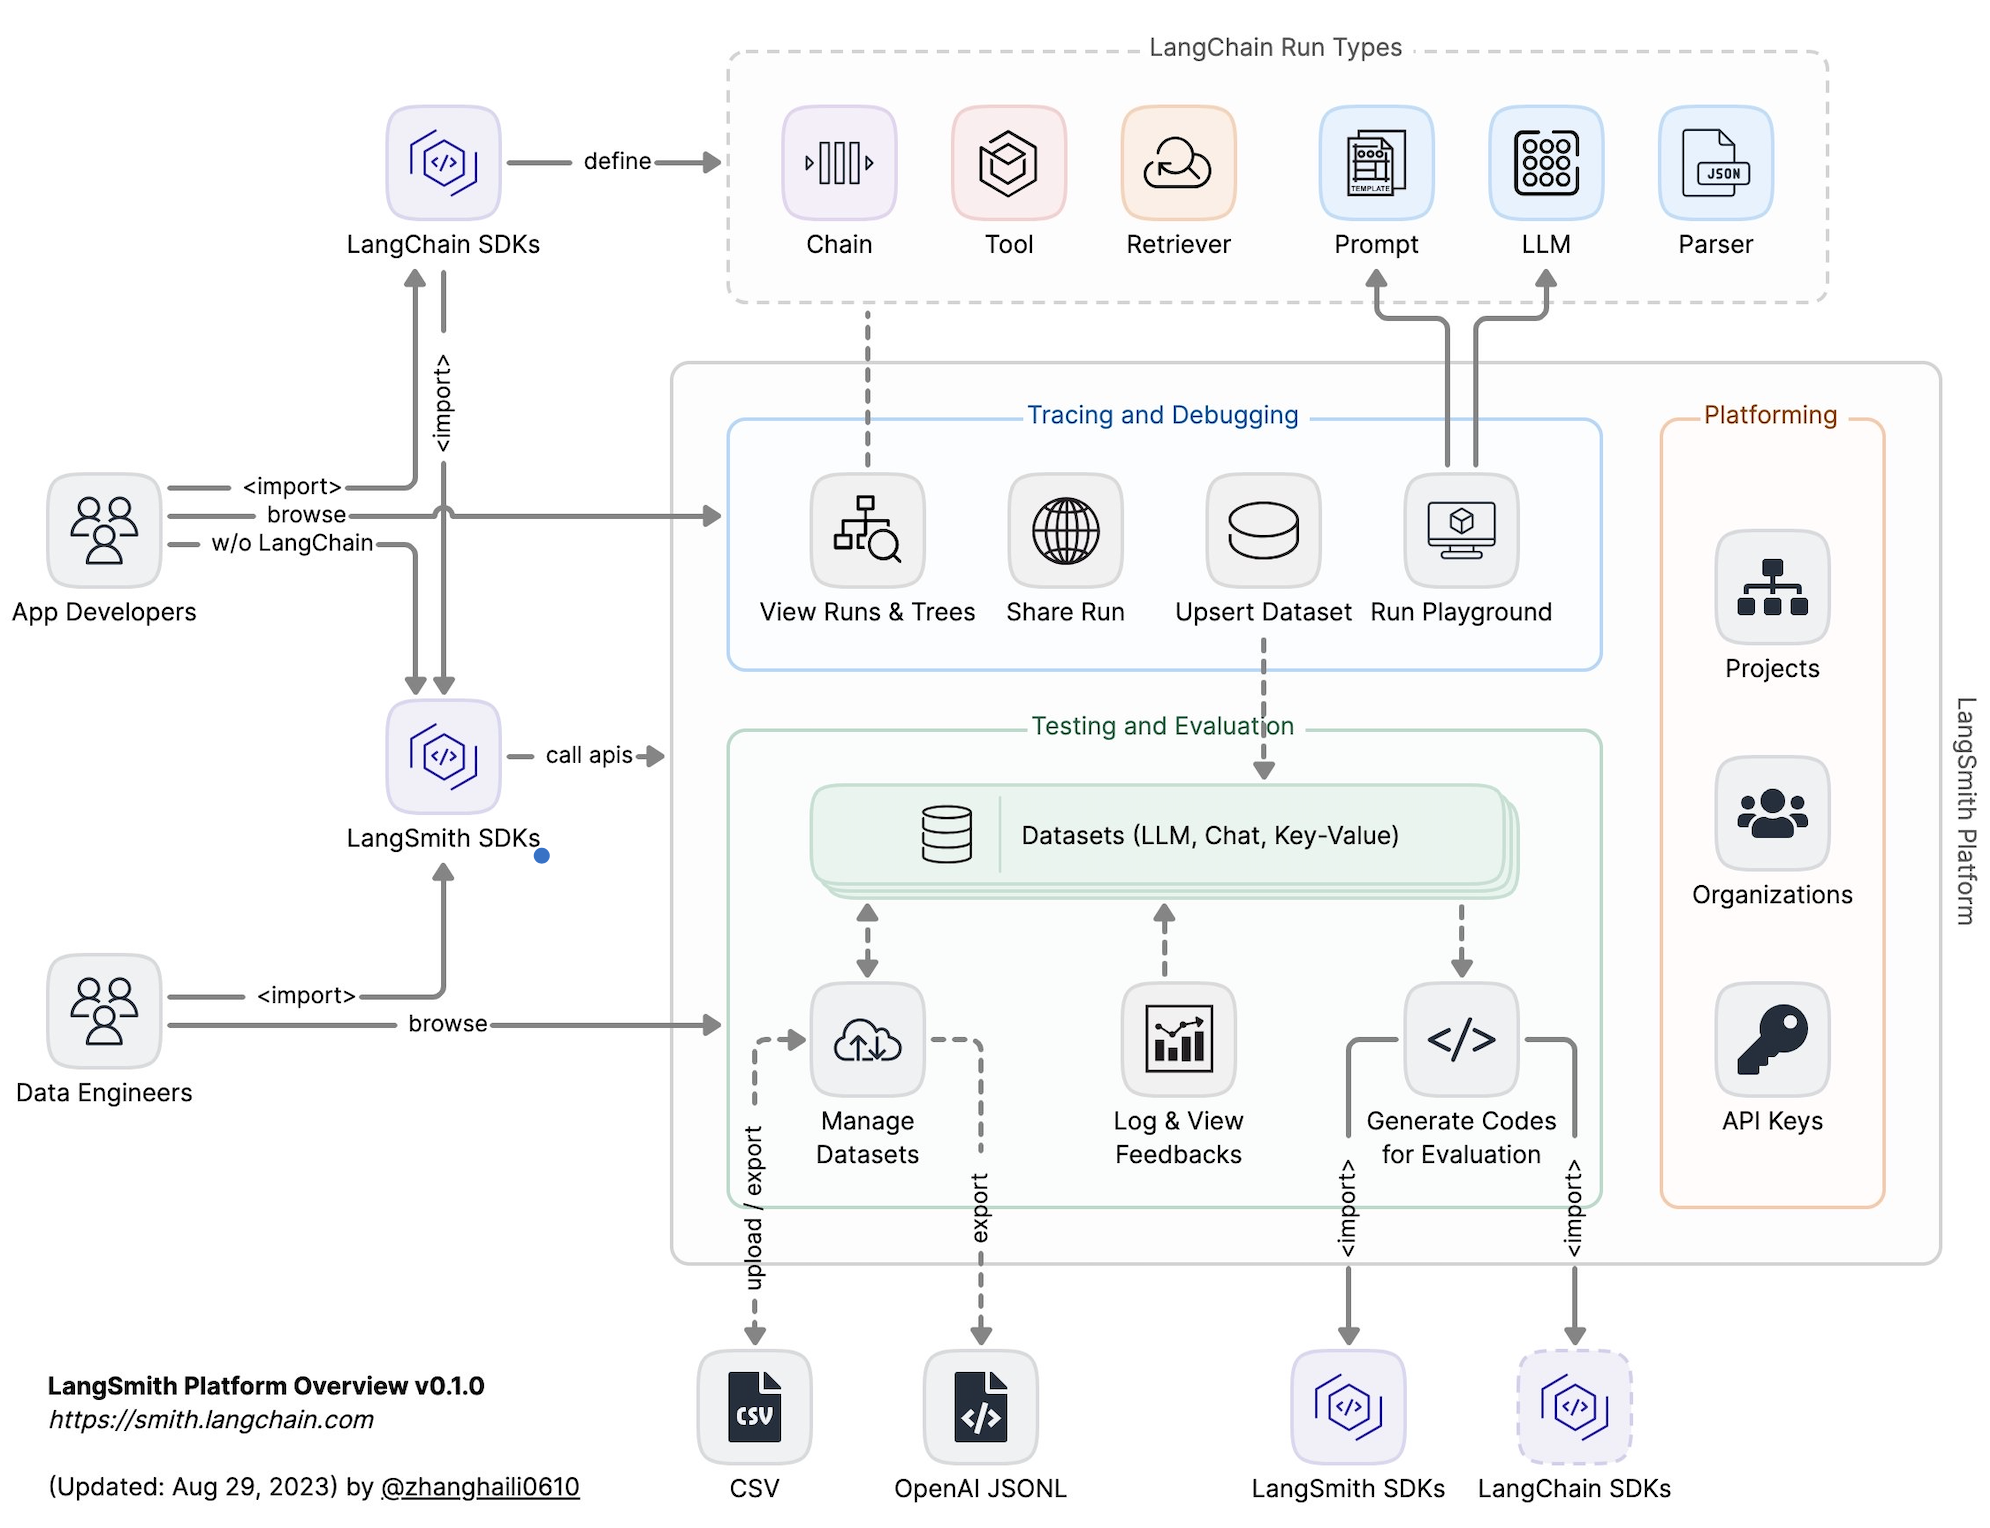
\includegraphics[width=0.9\textwidth]{Images/Langchain Architecture.png}
    \captionof{figure}{LangChain Architecture} \cite{langchainArchitecture}
    \label{fig:langchain_architecture}
\end{center}

Key features of LangChain include:
\begin{itemize}
    \item \textbf{Prompt Templates}: Facilitate the creation of dynamic prompts for LLMs.
    \item \textbf{Chains}: Enable the linking of multiple components to form a cohesive workflow.
    \item \textbf{Agents}: Allow for decision-making capabilities by selecting appropriate actions based on user input.
    \item \textbf{Memory}: Maintain context across interactions to support stateful conversations.
\end{itemize}

\subsubsection{LangGraph: Graph-Based Workflow Orchestration}
Building upon the foundations of LangChain, LangGraph introduces a graph-based approach to workflow orchestration, allowing for the modeling of complex, non-linear, and cyclical processes. In LangGraph, workflows are represented as directed graphs comprising nodes (representing operations or agents) and edges (defining the flow between nodes). This structure is particularly advantageous for applications requiring iterative processing, conditional branching, and multi-agent coordination.

\begin{center}
    \centering
    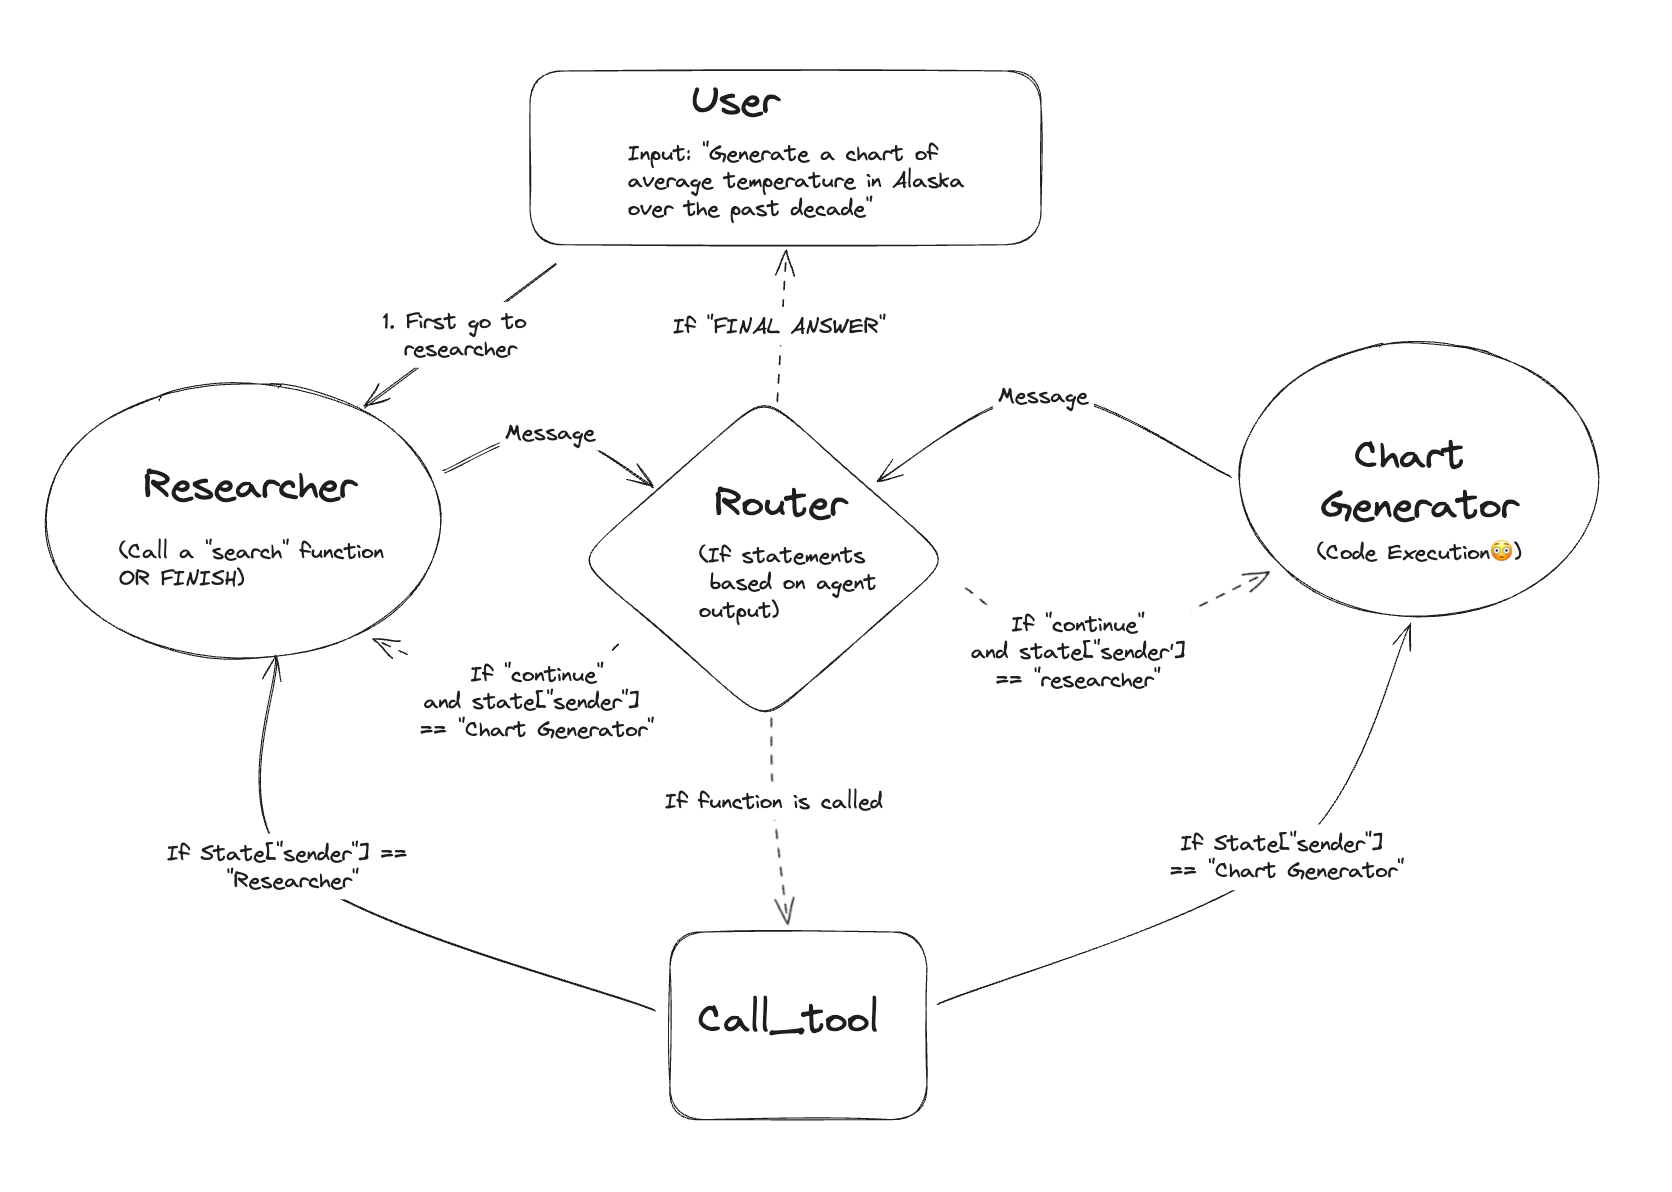
\includegraphics[width=0.9\textwidth]{Images/langgraph_mutil_agent.png}
    \captionof{figure}{LangGraph: Multi-Agent Workflows} \cite{langgraphMultiAgent}
    \label{fig:langgraph_multi_agent}
\end{center}

Notable capabilities of LangGraph include:
\begin{itemize}
    \item \textbf{Cyclic Workflows}: Support for loops and iterative processes within workflows.
    \item \textbf{Conditional Routing}: Dynamic decision-making to determine the next node based on runtime conditions.
    \item \textbf{State Management}: Persistent tracking of the system’s state throughout the workflow execution.
    \item \textbf{Multi-Agent Collaboration}: Facilitation of interactions between multiple agents, each with specialized roles.
\end{itemize}

\subsubsection{Comparative Analysis}
While both LangChain and LangGraph are designed to streamline the development of LLM-powered applications, they cater to different complexity levels and use cases. LangChain’s linear and modular approach is well-suited for straightforward tasks with a clear sequence of operations. In contrast, LangGraph’s graph-based architecture excels in scenarios requiring complex control flows, such as applications with iterative loops, conditional logic, or collaborative agent interactions.

\begin{table}[ht!]
    \centering
    \small
    \begin{tabularx}{\textwidth}{|l|X|X|}
        \hline
        \textbf{Feature} & \textbf{LangChain} & \textbf{LangGraph} \\
        \hline
        Workflow Structure & Sequential chains & Dynamic graphs \\
        Complexity Handling & Simple/moderate workflows & Moderate/complex workflows \\
        Iterative Processing & Limited & Fully supported (loops) \\
        Conditional Logic & Basic conditions & Advanced conditions \\
        Multi-Agent Coordination & Basic support & Robust collaboration \\
        State Management & Basic retention & Advanced tracking \\
        Use Case Suitability & Straightforward tasks & Complex adaptive tasks \\
        Flexibility & Rigid structure & Highly flexible \\
        Debugging and Monitoring & Good support & Enhanced visibility \\
        Real-time Decision Making & Limited & Extensive support \\
        Ideal Applications & Simple Q\&A, summarization & Complex multi-agent apps \\
        \hline
    \end{tabularx}
    \caption{Comparison of LangChain and LangGraph}
    \label{tab:langchain_langgraph_comparison}
\end{table}

\subsubsection{Conclusion}
LangChain and LangGraph offer robust frameworks for developing applications that leverage the capabilities of LLMs. The choice between them hinges on the complexity and requirements of the intended application. For linear and relatively simple workflows, LangChain provides an efficient and straightforward solution. Conversely, for applications necessitating complex control flows, iterative processing, and multi-agent coordination, LangGraph presents a more suitable architecture.

% Langfuse and Observability
\subsection{Langfuse and Observability}

% Overview
\subsubsection{Overview}
Langfuse is an open-source observability platform designed specifically for applications powered by Large Language Models (LLMs). It provides developers with tools to trace, debug, and analyze the behavior of LLM applications, ensuring better performance and reliability.

\begin{center}
    \centering
    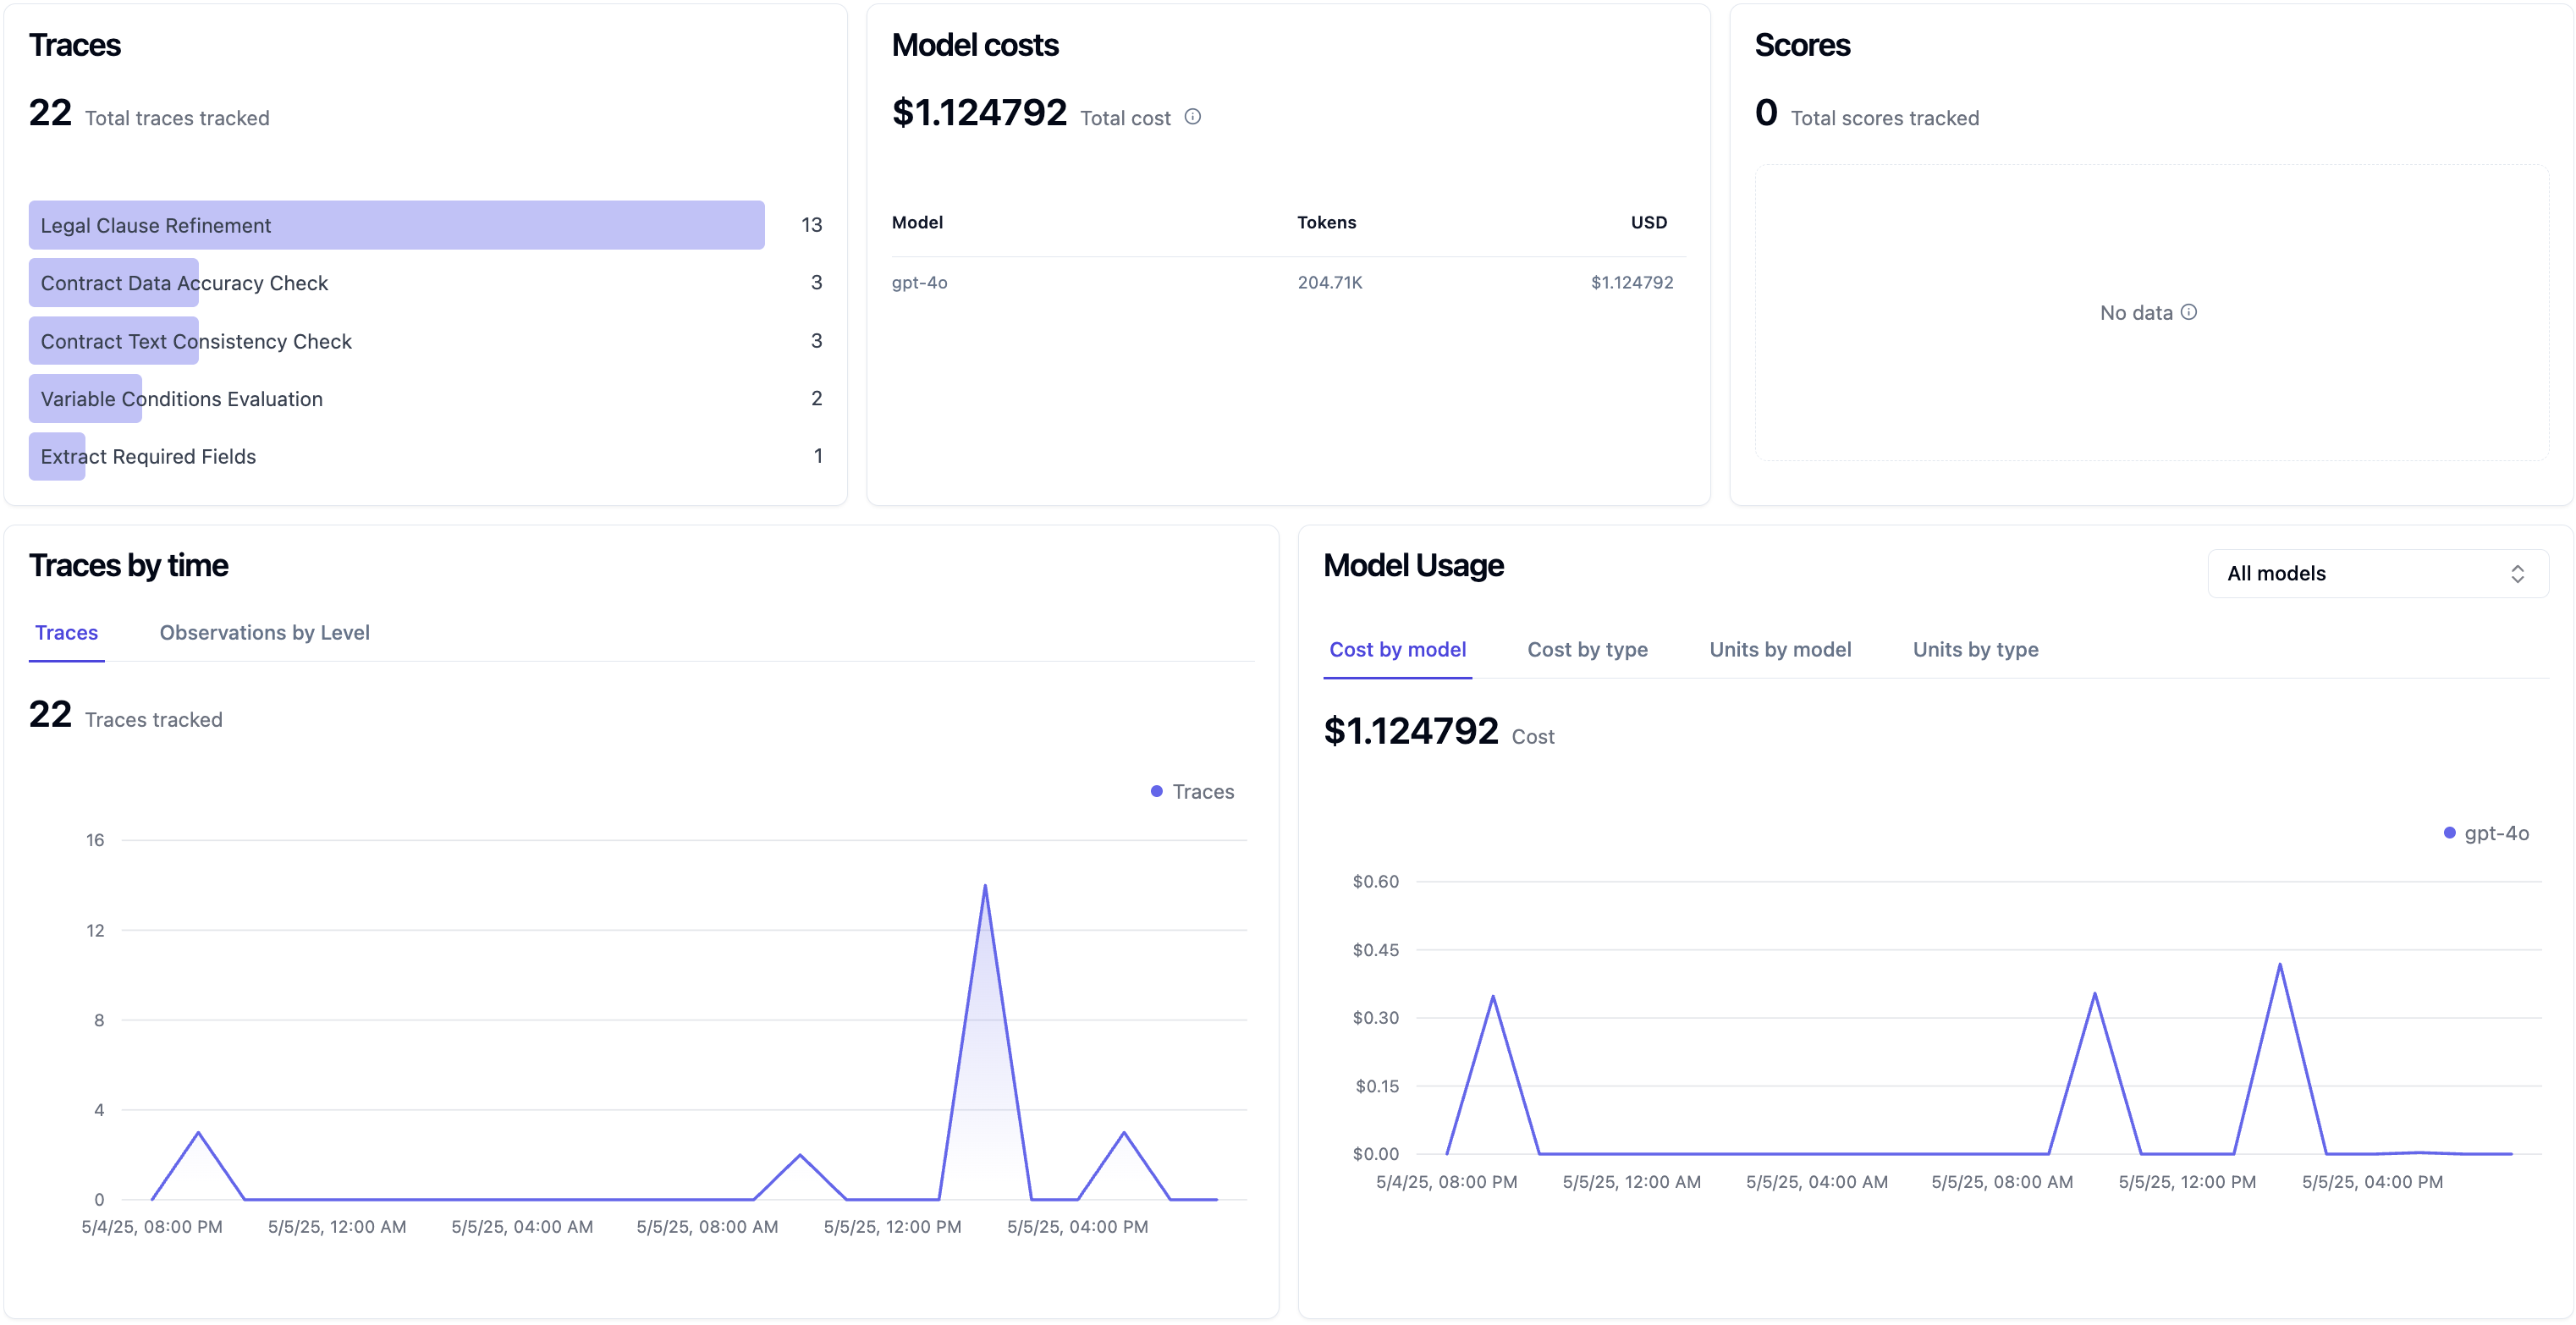
\includegraphics[width=1\textwidth]{Images/Langfuse Overview.png}
    \captionof{figure}{Langfuse Dashboard} \cite{langfuseDashboard}
    \label{fig:langfuseDashboard}
\end{center}

% Key Features
\subsubsection{Key Features}
\begin{itemize}
    \item \textbf{Comprehensive Tracing}: Langfuse captures detailed traces of LLM operations, including prompts, responses, and intermediate steps, allowing developers to understand the flow of data and identify issues effectively.
    \item \textbf{Session Management}: It groups related interactions into sessions, providing a holistic view of multi-turn conversations or complex workflows.
    \item \textbf{Analytics Dashboard}: Langfuse offers dashboards that display metrics such as latency, token usage, and cost, enabling teams to monitor and optimize application performance.
    \item \textbf{Prompt Management}: The platform includes tools for managing and versioning prompts, facilitating experimentation and iterative development.
    \item \textbf{Integration Support}: Langfuse integrates seamlessly with popular frameworks like LangChain, LlamaIndex, and OpenAI SDKs, as well as supports OpenTelemetry for broader observability needs.
\end{itemize}

% Deployment Options
\subsubsection{Deployment Options}
Langfuse can be deployed in various environments:

\begin{itemize}
    \item \textbf{Cloud Hosting}: Utilize Langfuse’s managed cloud service for quick setup and scalability.
    \item \textbf{Self-Hosting}: Deploy Langfuse on-premises or in private clouds using Docker, providing full control over data and configurations.
\end{itemize}

% Use Cases
\subsubsection{Use Cases}
\begin{itemize}
    \item \textbf{Debugging Complex Workflows}: By tracing each step of LLM operations, developers can pinpoint and resolve issues in complex applications.
    \item \textbf{Performance Monitoring}: Track metrics to identify bottlenecks and optimize resource usage.
    \item \textbf{Quality Assurance}: Analyze user interactions and feedback to improve response quality and user satisfaction.
    \item \textbf{Compliance and Auditing}: Maintain detailed logs for auditing purposes, ensuring compliance with regulatory standards.
\end{itemize}

% Conclusion
\subsubsection{Conclusion}
Incorporating Langfuse into the development lifecycle of LLM applications enhances transparency, reliability, and efficiency, making it an invaluable tool for teams aiming to build robust AI solutions.

% Tiptap for Rich Text Editing
\subsection{Tiptap for Rich Text Editing}

% Overview
\subsubsection{Overview}
Tiptap is a headless, open-source rich text editor framework built on ProseMirror, designed for developers seeking full control over their content editing interfaces. Its modular architecture and extensive extension ecosystem make it a powerful tool for building customized, collaborative, and AI-enhanced editing experiences.

\begin{center}
    \centering
    
\includegraphics[width=0.8\textwidth]{Images/Tiptap editor.jpg}
    \captionof{figure}{Tiptap Editor} \cite{tiptap}
    \label{fig:tiptap}
\end{center}

% Architecture and Core Concepts
\subsubsection{Architecture and Core Concepts}
Tiptap is a headless, framework-agnostic rich text editor built on top of ProseMirror, designed to provide developers with full control over the editor’s functionality and appearance. Its architecture is modular and extensible, allowing for the creation of customized editing experiences.

\begin{center}
    \centering
    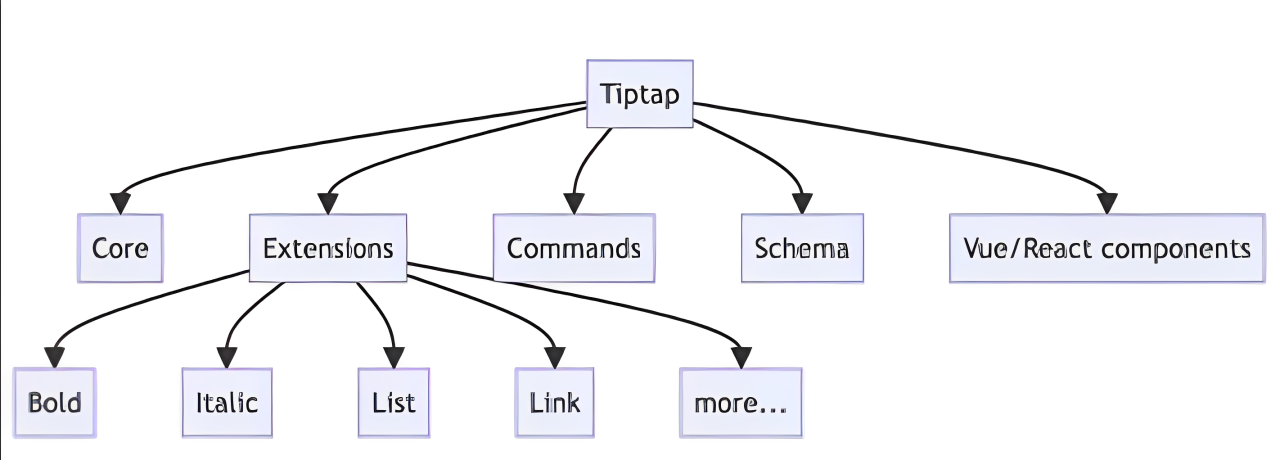
\includegraphics[width=0.8\textwidth]{Images/Tiptap Architecture.png}
    \captionof{figure}{Tiptap Architecture} \cite{tiptapArchitecture}
    \label{fig:tiptapArchitecture}
\end{center}

Key Architectural Components:
\begin{itemize}
    \item \textbf{Schema}: Defines the structure of the document, specifying the allowed nodes (e.g., paragraphs, headings) and marks (e.g., bold, italic). This strict schema ensures content consistency and predictability.
    \item \textbf{State}: Represents the current content and selection within the editor. It is immutable and updated through transactions, enabling features like undo/redo and collaborative editing.
    \item \textbf{Transaction}: Encapsulates changes to the state, such as text insertions or formatting. Transactions ensure that state changes are predictable and manageable.
    \item \textbf{Extensions}: Modular units that add functionality to the editor, such as new nodes, marks, commands, or plugins. Tiptap provides a rich set of core and community extensions, and developers can create custom ones as needed.
    \item \textbf{Commands}: Functions that perform actions within the editor, often used to manipulate the document or respond to user input. Commands can be chained for complex operations.
\end{itemize}

% Key Features
\subsubsection{Key Features}
\begin{itemize}
    \item \textbf{Extension-Based Modularity}: Tiptap offers over 100 extensions, including both open-source and Pro options, allowing developers to tailor the editor’s functionality to specific needs.
    \item \textbf{Real-Time Collaboration}: Through integrations like Hocuspocus and CRDTs, Tiptap supports collaborative editing with features like live cursors and offline synchronization.
    \item \textbf{AI Integration}: The Content AI extension enables in-editor AI capabilities such as text suggestions, translations, and content generation, enhancing the writing experience.
    \item \textbf{Framework Agnostic}: Tiptap’s design allows it to be integrated into various JavaScript frameworks, providing flexibility in application development.
\end{itemize}

% Use Cases
\subsubsection{Use Cases}
Tiptap is suitable for a wide range of applications, including:
\begin{itemize}
    \item Building Notion-like editors with custom blocks and interactions.
    \item Developing collaborative document editing platforms.
    \item Creating AI-assisted writing tools with real-time suggestions.
    \item Implementing rich text editors in CMS platforms. 
\end{itemize}    

% Conclusion
\subsubsection{Conclusion}
Tiptap stands out as a versatile and developer-friendly rich text editor framework. Its combination of headless architecture, modular extensions, and support for real-time collaboration and AI integration makes it a compelling choice for modern web applications requiring customized content editing solutions.

% Project Requirements
\section{Specification of Requirements}
Given the agile nature of the project, the actors as well as functional and non-functional requirements are subject to evolve. The elements below reflect the current state of the project.

% Business Architecture
\subsection{Business Architecture}
The business architecture depicted in Figure~\ref{fig:business_architecture} outlines the overarching structure and planned components of the intelligent contract management platform. The platform integrates three main components supported by robust underlying layers of data management, security, observability, and tool integration capabilities.

\begin{center}
    \centering
    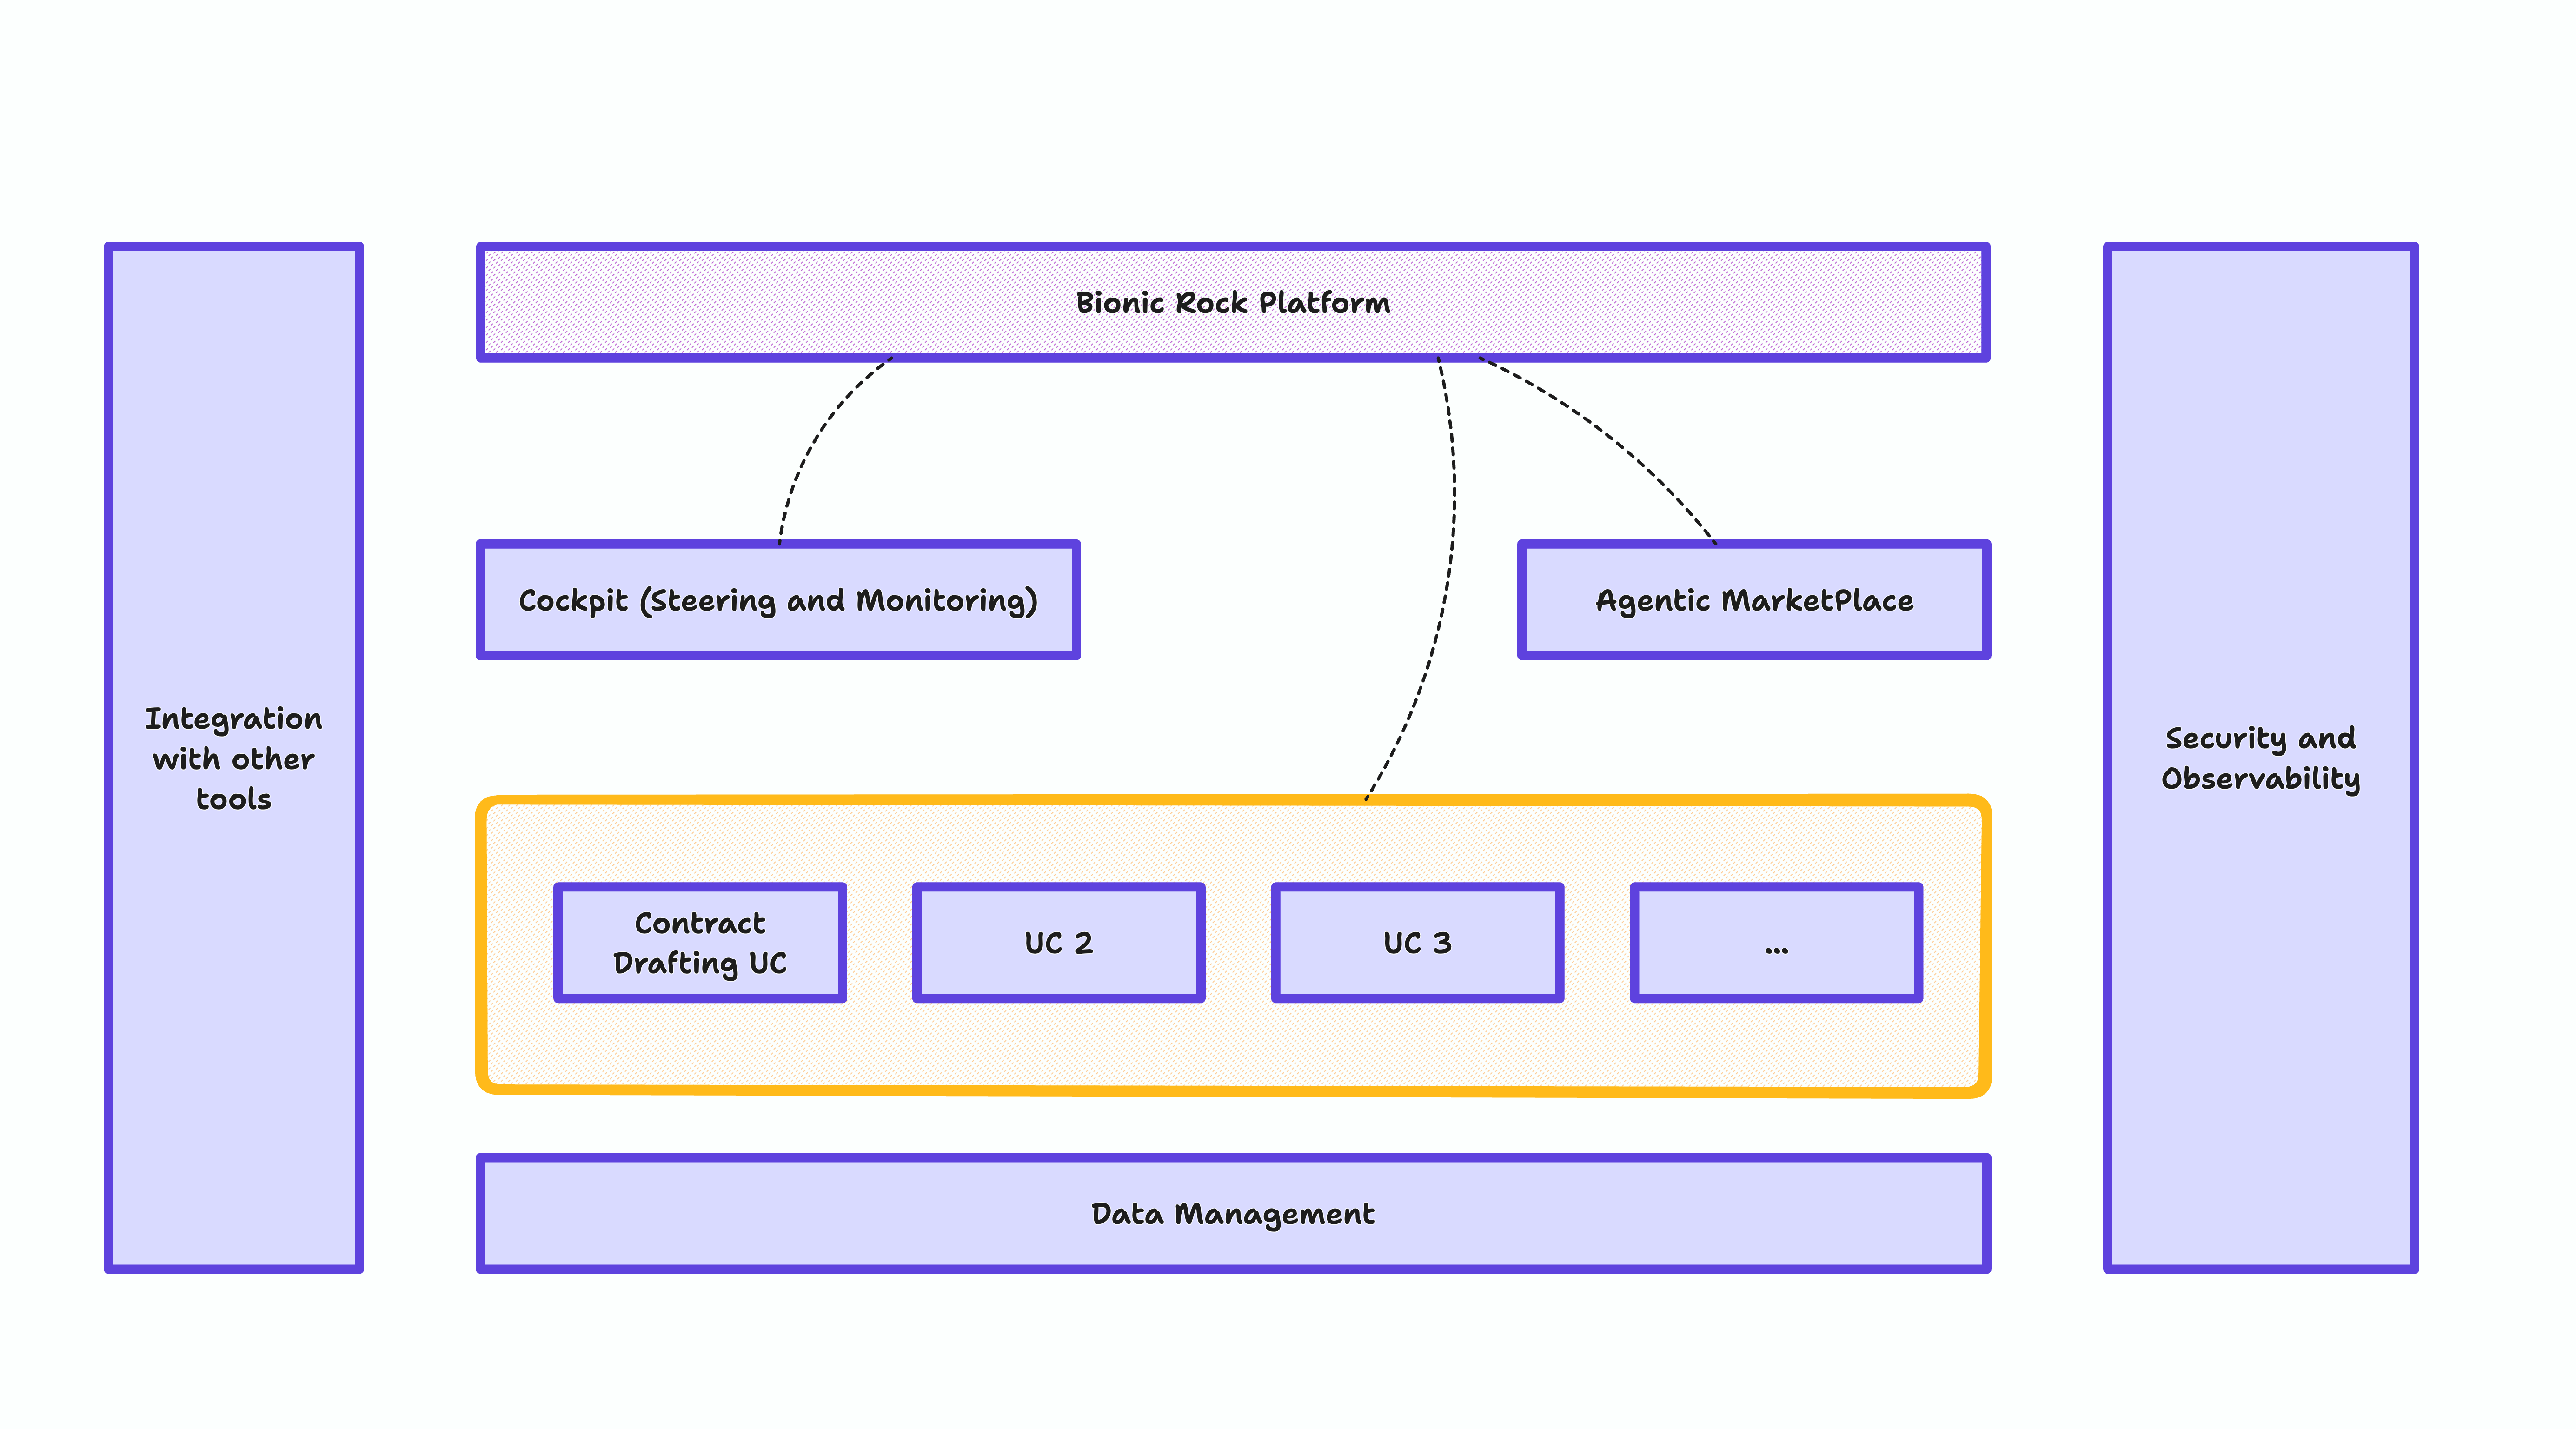
\includegraphics[width=0.9\textwidth]{Images/Business Architecture.png}
    \captionof{figure}{Business Architecture Overview} \cite{business_architecture}
    \label{fig:business_architecture}
\end{center}

The platform structure is organized into three core areas:

\begin{itemize}
\item \textbf{Cockpit (Steering and Monitoring)}: This area provides oversight and real-time analytics, enabling stakeholders to monitor system performance, track usage, and manage workflows effectively.
\item \textbf{Agentic Marketplace}: Designed to host various autonomous AI agents, this component facilitates the scalable deployment and orchestration of intelligent services, supporting diverse, dynamic business needs and agent interactions.
\item \textbf{Use Case Features}: These represent modular functionalities tailored to specific business processes. The primary use case currently prioritized is the \textbf{Contract Drafting Use Case (UC)}, scheduled for completion within a 21-week timeframe. This use case is central to my internship project and focuses on automating and enhancing the contract drafting process through intelligent clause selection, AI-assisted drafting, compliance verification, and collaboration enhancements.
\end{itemize}

These foundational components are encapsulated within a broader environment of:

\begin{itemize}
\item \textbf{Data Management}: Ensures consistent data governance, quality, and efficient access to support the platform's intelligent features.
\item \textbf{Integration with Other Tools}: Provides seamless interoperability with external and internal enterprise applications, extending the platform's capabilities and ensuring a cohesive user experience.
\item \textbf{Security and Observability}: Delivers comprehensive security measures and observability tools to protect data integrity, ensure compliance, and provide transparent system monitoring and diagnostics.
\end{itemize}

This structured business architecture aims to offer a scalable, secure, and integrative platform capable of addressing complex legal operations through advanced technological solutions.

% Actor Identification
\subsection{Actor Identification}
An actor specifies a role played by a user or any other system interacting with the solution. Actors are always external to the system, interacting by initiating a use case, providing inputs, or receiving outputs. In the context of our platform, we have two types of actors:

\begin{table}[ht!]
    \centering
    \small
    \begin{tabularx}{\textwidth}{|l|X|}
        \hline
        \textbf{Actor} & \textbf{Role} \\
        \hline
        Sales User & Responsible for creating and managing contract documents and negotiations with clients. \\
        Legal User & Oversees contract compliance, manages legal clauses, and reviews contracts. \\
        Administrator & Manages platform users, roles, permissions, and oversees system configurations. \\
        \hline
    \end{tabularx}
    \caption{Actors and Their Roles}
    \label{tab:actorsWithRoles}
\end{table}

% Functional Requirements
\subsection{Functional Requirements}

% Authentication
\subsubsection{Authentication}
The system must allow users to authenticate using Azure Entra ID credentials.

% Sales User Functionalities
\subsubsection{Sales User Functionalities}

\textbf{Contract Generation}:
\begin{itemize}
\item Initiate contract drafting using text input, voice transcription, or document upload.
\item Verify client information from historical data.
\item Select and adjust template inputs (Incoterm, Contract Type, Product).
\item Adjust variables like price and volume.
\item Generate final contract draft and move to editing mode.
\end{itemize}

\textbf{Contract Editing}:
\begin{itemize}
\item Access a rich-text editor (Tiptap-based).
\item Track changes across versions.
\item Request additional legal clauses.
\item Access versioning of contracts.
\item Modify variables in the contracts (data mapping panel).
\item Request clauses to be added, modified, or deleted.

\end{itemize}

\textbf{Contract Review \& Compliance}:
\begin{itemize}
\item Trigger AI-powered compliance checks (data accuracy, text consistency, legal compliance).
\item Receive detailed review summaries and recommendations.
\item Review contracts and change status (in editing, in review, finalized).
\end{itemize}

\textbf{Export, Sharing, and Management}:
\begin{itemize}
\item Export contracts as downloadable files (Word, PDF).
\item Share contracts via secure links or attachments in emails.
\item Access contracts in the contract repository.
\item Archive and delete contracts.
\end{itemize}

% Legal User Functionalities
\subsubsection{Legal User Functionalities}

\textbf{Clause Management}:
\begin{itemize}
\item Review clause addition requests from Sales.
\item Create, insert, modify, or delete legal clauses, either upon Sales requests or independently.
\item Utilize AI assistance to refine clause content.
\end{itemize}

\textbf{Contract Editing and Versioning}:
\begin{itemize}
\item Access and create versions of contracts.
\item Restore previous versions of contracts.
\item Edit contracts using a rich-text editor (Tiptap-based).
\item \item Modify variables in the contracts (data mapping panel).
\end{itemize}

\textbf{Contract Review \& Compliance}:
\begin{itemize}
\item Perform detailed legal compliance checks.
\item Verify mandatory clauses, annexes, and specifications.
\item Ensure legal alignment and minimize liabilities.
\item Review contracts and change status (in editing, in review, finalized).
\end{itemize}

\textbf{Export, Sharing, and Management}:
\begin{itemize}
\item Export contracts as downloadable files (Word, PDF).
\item Share contracts via secure links or attachments in emails.
\item Access contracts in the contract repository.
\end{itemize}

% Administrator Functionalities
\subsubsection{Administrator Functionalities}
\textbf{User Management}:
\begin{itemize}
    \item Add, modify, or remove platform users.
    \item Manage role-based permissions.
\end{itemize}

\textbf{System Configuration}:
\begin{itemize}
    \item Oversee integration settings, security configurations, and monitoring dashboards.
\end{itemize}

% Non-Functional Requirements
\subsection{Non-Functional Requirements}
\begin{itemize}
    \item \textbf{Usability}: The application should be intuitive, ensuring ease of use for Sales, Legal, and Admin users.
    \item \textbf{Maintainability}: The system should be modular and maintainable, supporting frequent updates.
    \item \textbf{Security}: Strict management of user access, data protection, and compliance with regulatory standards.
    \item \textbf{Performance}: Responsive interface, quick data retrieval, and AI analysis with low latency.
    \item \textbf{Scalability}: Easily scalable to support growing user base and additional functionalities.
\end{itemize}

% Use Case Diagram
\subsection{Use Case Diagram}
The Use Case Diagram presented in Figure~\ref{fig:use_case_diagram} visually represents the interactions between the identified actors—Sales Users, Legal Users, and Administrators—and the main functionalities offered by the intelligent contract management platform. It illustrates how each user group engages with distinct and shared system features, clearly depicting the overall workflow from contract drafting and editing to compliance verification, version control, and collaboration activities.

\begin{center}
    \centering
    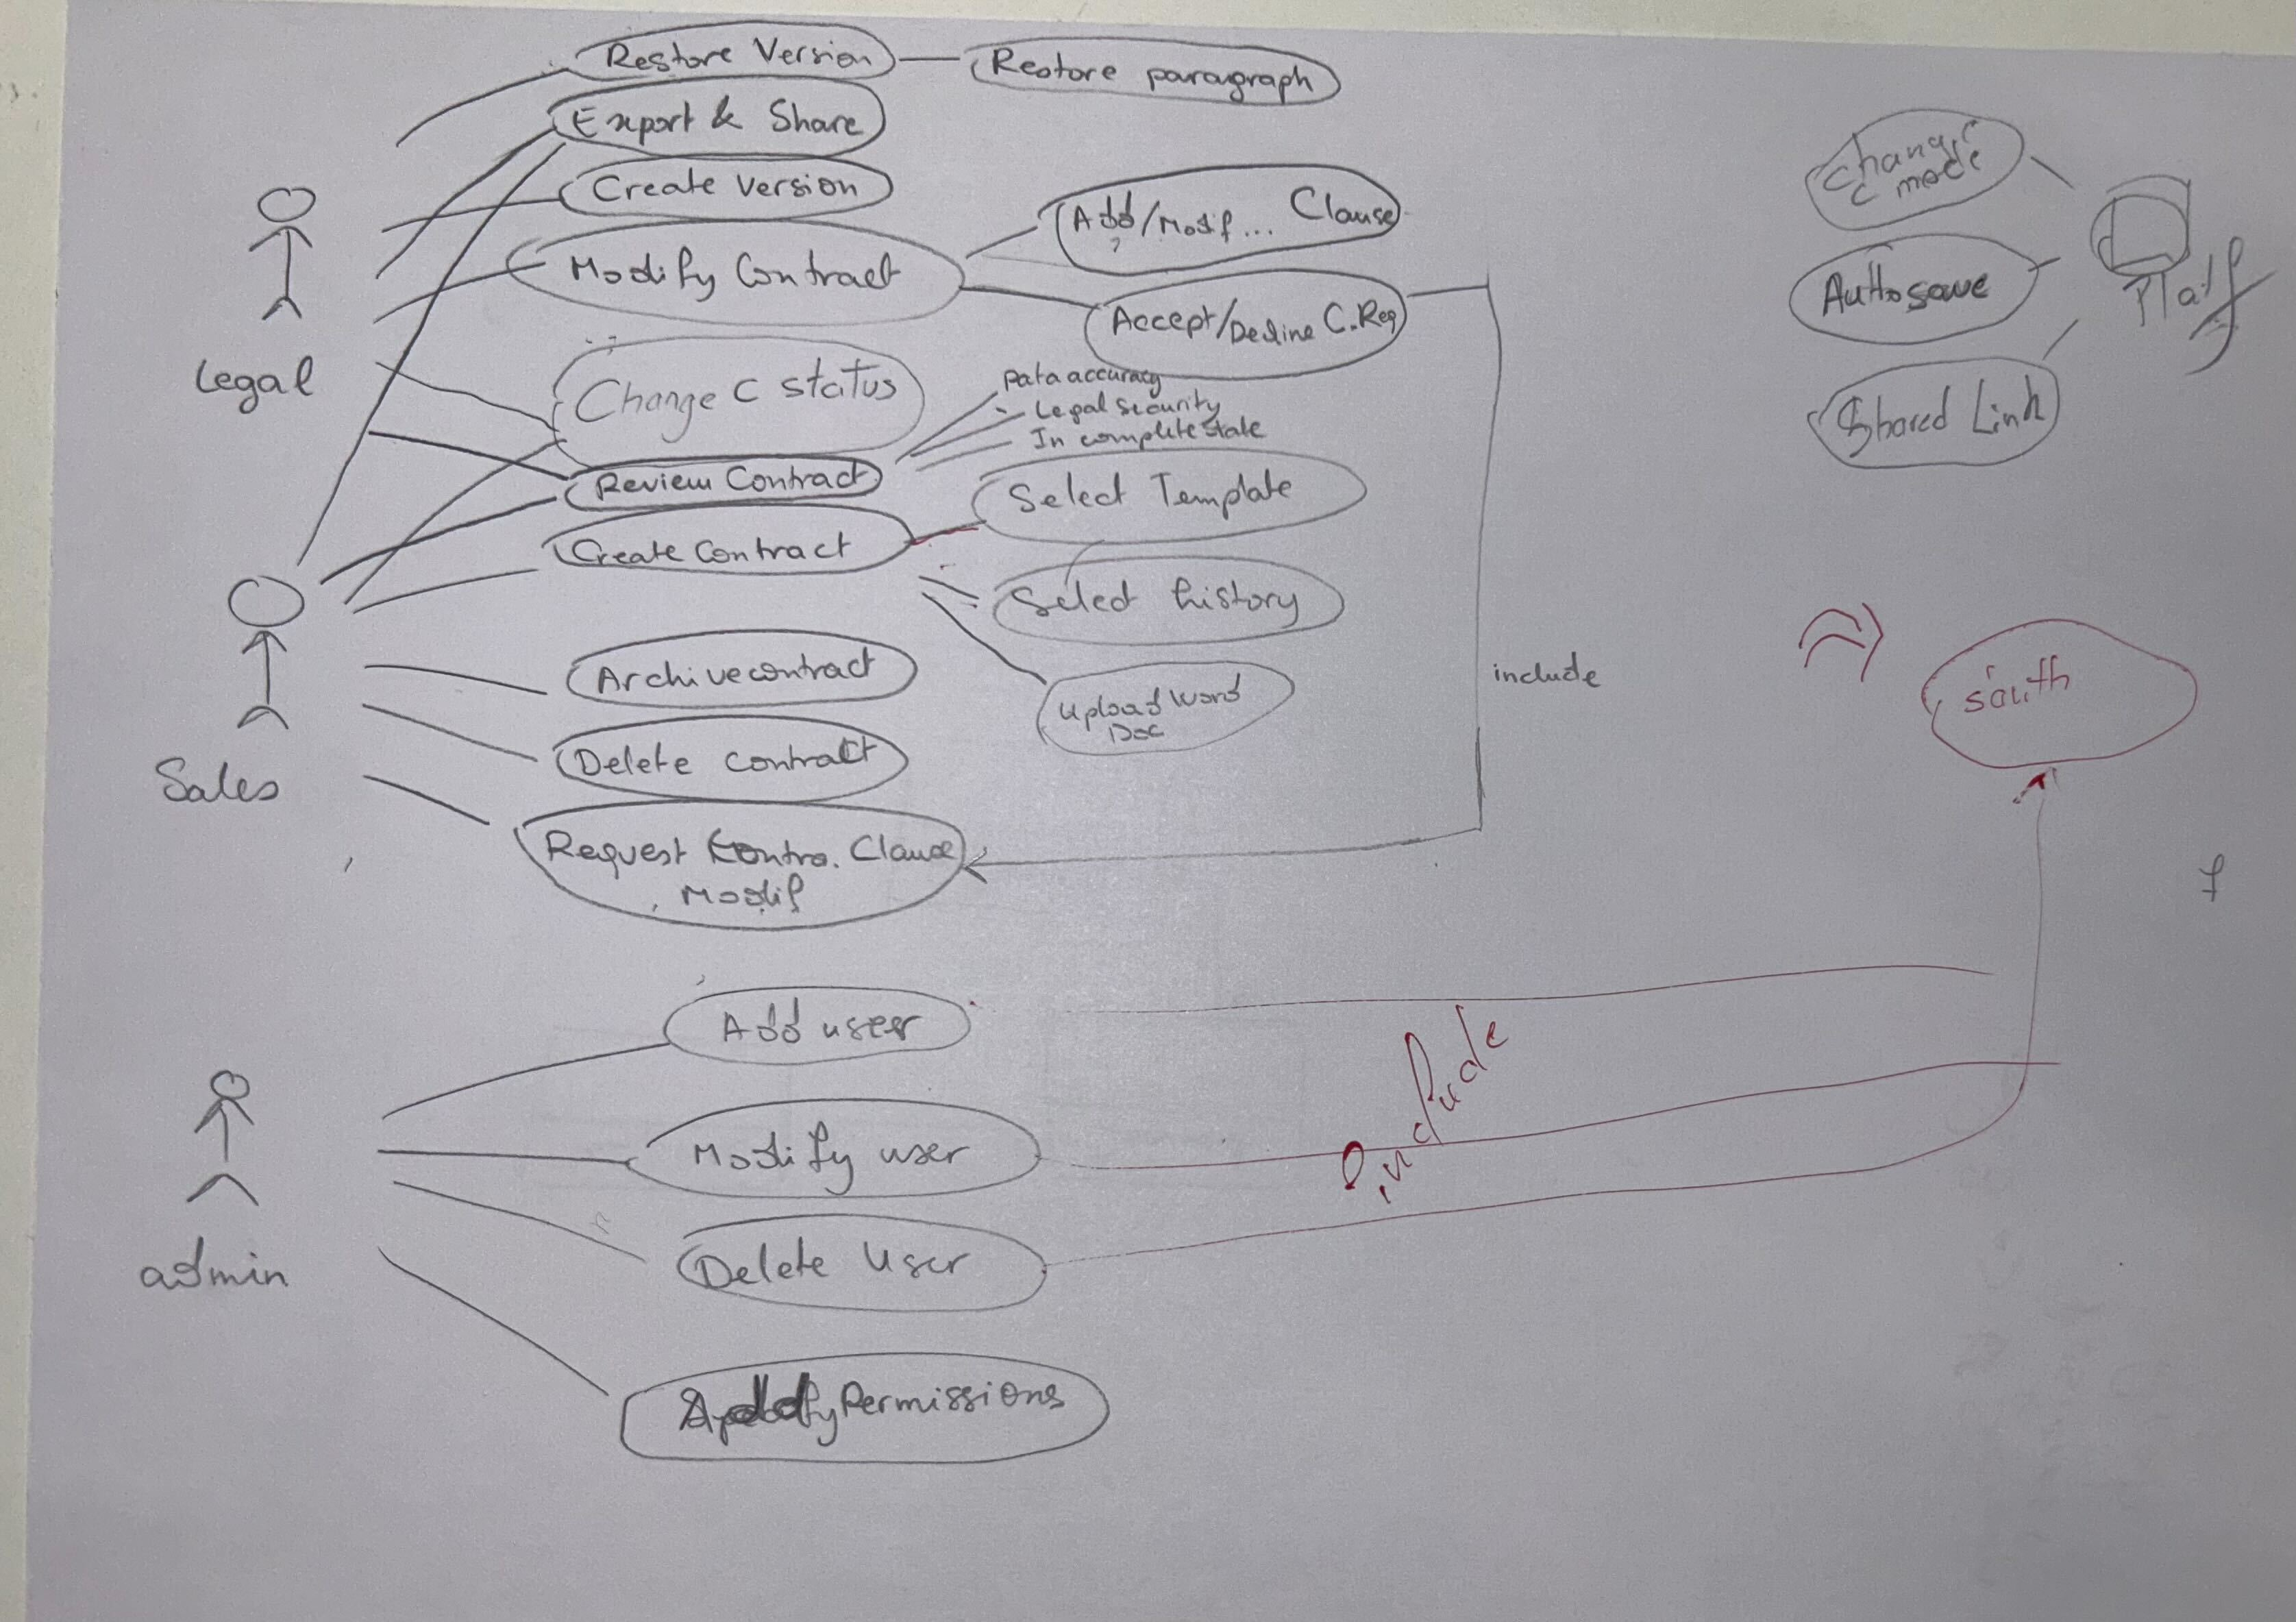
\includegraphics[width=0.9\textwidth]{Images/Use Case Diagram.jpg}
    \captionof{figure}{Use Case Diagram} \cite{use_case_diagram}
    \label{fig:use_case_diagram}
\end{center}

The diagram thus serves as a concise summary of system capabilities and user interactions, effectively capturing the essential scenarios envisaged within the platform’s scope. This visual representation provides a foundation for understanding user roles and their interactions, facilitating clear communication and alignment among stakeholders during the development and implementation of the platform.

% Textual Description
\subsection{Textual Description}

Pour décrire la dynamique d’un cas d’utilisation, il faut recenser toutes les interactions entre l’acteur et le système de façon textuelle. Cette description est indispensable, car elle permet de communiquer facilement avec les différentes parties prenantes et de s’entendre sur la terminologie métier employée.

\textbf{Textual Description of Use Case: Create Contract}

\begin{table}[ht!]
    \centering
    \small
    \begin{tabularx}{\textwidth}{|l|X|}
        \hline
        \textbf{Actor} & Sales User \\
        \hline
        \textbf{Goal} & Create a new contract \\
        \hline
        \textbf{Preconditions} & User must be authenticated \\
        \hline
        \textbf{Postconditions} & Successful creation of a contract draft \\
        \hline
        \textbf{Nominal Scenario} &
            1. User accesses the Contract Repository page. \\[3pt]
            2. User clicks on "Generate a New Contract." \\[3pt]
            3. User selects one of the following input methods: voice prompt, image upload, or text prompt. \\[3pt]
            4. System extracts key contract information. \\[3pt]
            5. If a new client or mismatched client information is detected, the system prompts the user for confirmation. \\[3pt]
            6. User confirms key information. \\[3pt]
            7. System automatically generates the contract step-by-step. \\
        \hline
        \textbf{Alternative Scenario} & Missing required information – Display an error message indicating the specific missing information. \\
        \hline
    \end{tabularx}
    \caption{Textual Description of Use Case: Create Contract}
    \label{tab:create_contract}
\end{table}

\textbf{Textual Description of Use Case: Review Contract}

\begin{table}[ht!]
    \centering
    \small
    \begin{tabularx}{\textwidth}{|l|X|}
        \hline
        \textbf{Actor} & Legal User or Sales User \\
        \hline
        \textbf{Goal} & Review a contract for accuracy, consistency, and legal security \\
        \hline
        \textbf{Preconditions} & User must be authenticated and in the Contract Editing page \\
        \hline
        \textbf{Postconditions} & Contract reviewed with provided suggestions and quality score \\
        \hline
        \textbf{Nominal Scenario} &
            1. User accesses the Editor View (Contract Editing page). \\[3pt]
            2. User selects "Review" in the right panel. \\[3pt]
            3. User chooses between "Accuracy and Consistency" and "Legal Security" review options. \\[3pt]
            4. User initiates the review process. \\[3pt]
            5. System completes the review and provides a quality score (\%). \\[3pt]
            6. System presents suggestions generated by the LLM for the user to accept or discard. \\
        \hline
        \textbf{Alternative Scenario} & Review fails or incomplete – System displays a message indicating the review error and required next steps. \\
        \hline
    \end{tabularx}
    \caption{Textual Description of Use Case: Review Contract}
    \label{tab:review_contract}
\end{table}

\textbf{Textual Description of Use Case: Create Clause Request}

\begin{table}[ht!]
    \centering
    \small
    \begin{tabularx}{\textwidth}{|l|X|}
        \hline
        \textbf{Actor} & Sales User \\
        \hline
        \textbf{Goal} & Create a clause request to add, modify, or delete clauses \\
        \hline
        \textbf{Preconditions} & User must be authenticated and on the Contract Editing page \\
        \hline
        \textbf{Postconditions} & Clause request submitted and pending Legal User action \\
        \hline
        \textbf{Nominal Scenario} &
            1. User accesses the Contract Editing page.\\[3pt]
            2. User initiates a clause request from the left panel in the clause area or by right-clicking on an article, clause, or sub-clause.\\[3pt]
            3. User enters the description of the request.\\[3pt]
            4. User optionally refines the request description using an LLM-powered "Refine" button.\\[3pt]
            5. User submits the clause request.\\[3pt]
            6. Legal User receives the request and decides to accept or reject it.\\[3pt]
            7. If accepted, Legal User creates, modifies, or deletes the relevant articles or clauses.\\
        \hline
        \textbf{Alternative Scenario} & Invalid or incomplete request – System displays an error message indicating required corrections. \\
        \hline
    \end{tabularx}
    \caption{Textual Description of Use Case: Create Clause Request}
    \label{tab:create_clause_request}
\end{table}

% Analysis Sequence Diagram
\subsection{Analysis Sequence Diagram}
To clearly understand the chronological interactions between the system and its actors, analysis sequence diagrams are utilized. These diagrams illustrate the exchanges required between actors and the system to achieve a specific use case, facilitating a comprehensive understanding of the process flow and interactions involved.

\begin{center}
    \centering
    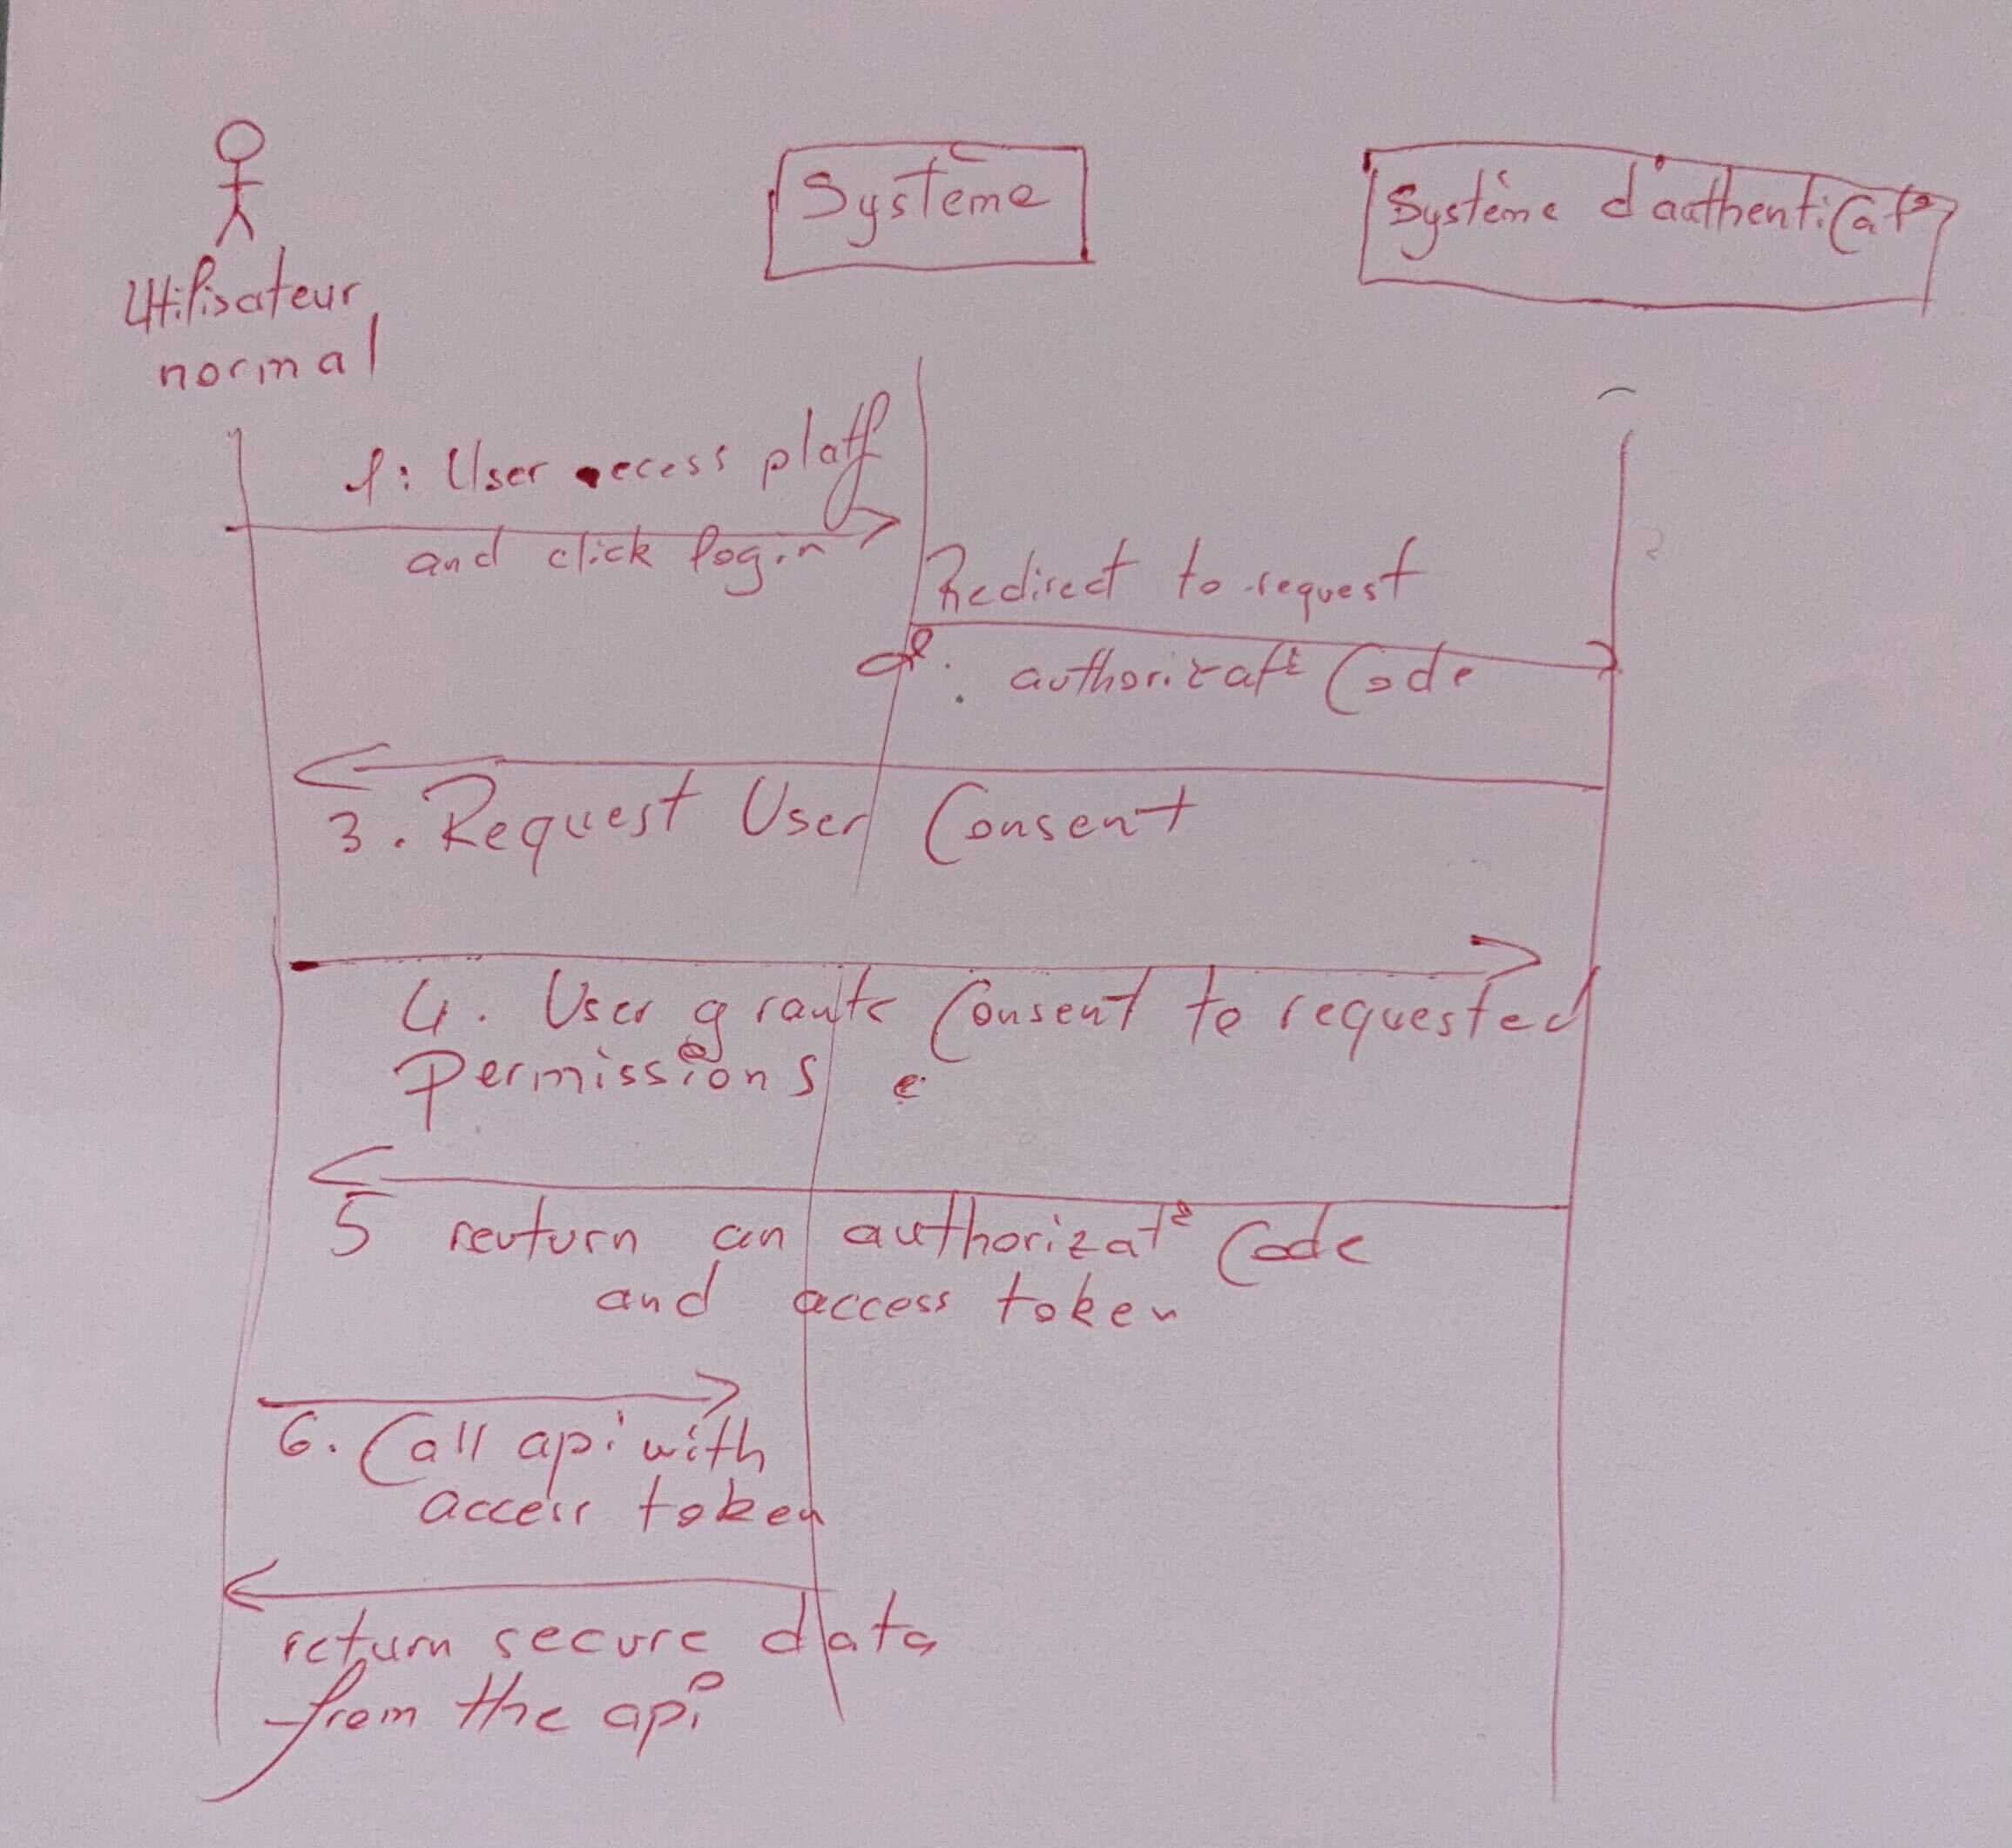
\includegraphics[width=0.8\textwidth]{Images/Analysis Sequence Diagram.jpg}
    \captionof{figure}{Analysis Sequence Diagram} \cite{analysis_sequence_diagram}
    \label{fig:analysis_sequence_diagram}
\end{center}

The diagram presented above outlines the interaction flow between a normal user intending to authenticate, the main system, and an external authentication system. Initially, the user accesses the platform and clicks on the login button, which prompts the system to redirect the authentication request to the external authentication system. The external authentication system then requests user consent for specific permissions. Upon granting consent by the user, the authentication system issues an authorization code along with an access token back to the system. Finally, the system utilizes this access token to securely call the API and retrieve the requested secured data.

% Constraints and Assumptions
\subsection{Constraints and Assumptions}
To clearly delineate the operational environment and development boundaries, the following constraints and assumptions have been identified:

\textbf{Constraints:}
\begin{itemize}
    \item \textbf{Enterprise Security Compliance}: The system must strictly comply with the organization’s security policies, standards, and regulatory frameworks, ensuring the protection and confidentiality of sensitive contractual and user information.
    \item \textbf{Infrastructure Compatibility}:All technical solutions must be compatible with existing enterprise systems, particularly Azure-based services such as Azure Kubernetes Service (AKS), Azure Entra ID, and Azure PostgreSQL, to ensure seamless integration and minimize disruptions.
    \item \textbf{Cost Efficiency}:The platform must be developed and operated within the allocated budget constraints, adhering to the capacity planning forecasts to optimize resource utilization and cost-effectiveness.
    \item \textbf{System Scalability}:The solution must accommodate future growth without significant re-engineering, enabling smooth onboarding of additional functionalities, agents, and user groups.
\end{itemize}

\textbf{Assumptions:}
\begin{itemize}
    \item \textbf{Data Availability and Quality}: It is assumed that structured and high-quality data is consistently available from internal sources and third-party integrations to ensure effective AI-driven decision-making.
    \item \textbf{Reliable Cloud Infrastructure}: It is assumed that the Azure cloud infrastructure provides continuous, high-performance service with minimal downtime, ensuring uninterrupted user experiences and workflows.
    \item \textbf{Stable Internet Connectivity}: It is assumed that end users have stable and continuous internet connectivity, enabling consistent access to cloud-hosted services.
    \item \textbf{User Proficiency}: Users are assumed to have a basic level of digital proficiency, enabling them to interact effectively with the intuitive yet sophisticated interfaces provided by the system.
    \item \textbf{Stakeholder Collaboration}: Continuous engagement from all stakeholders, including legal experts, technical teams, and business users, is expected to ensure alignment and smooth progression throughout the project’s lifecycle.
\end{itemize}

% Conclusion
\section{Conclusion}
This chapter outlined the analytical and technical specifications of the intelligent contract management platform. By presenting detailed UML diagrams, including use case and sequence diagrams, the interactions and functionalities of the system were concisely represented. Together with clearly defined requirements and the outlined project architecture, these elements provide a robust foundation for successful implementation.